\documentclass[10pt,letterpaper,notitlepage]{article}
\usepackage[utf8]{inputenc}
\usepackage{amsmath}
\usepackage{amsfonts}
\usepackage{amssymb}
\usepackage{graphicx}
\usepackage{cancel}
\usepackage{float}
\usepackage{cite}
\usepackage{fancyvrb}

\usepackage[ruled,vlined]{algorithm2e}


\usepackage[left=0.75in, right=0.75in, bottom=1.0in,top=0.75in]{geometry}

%\usepackage{caption} 
%\captionsetup[table]{skip=10pt}
%\usepackage[font=small,labelfont=bf]{caption}

\usepackage{comment}
\usepackage{listings}

\usepackage{color}


\usepackage{multicol}

\usepackage{appendix}

\usepackage{fancyhdr}
%\usepackage[colorlinks=true,linkcolor=blue,urlcolor=black,bookmarksopen=true,bookmarks]{hyperref}
\usepackage{bookmark}
\hypersetup{%
	pdfborder = {0 0 0}
}

\usepackage{multicol}
\setlength{\columnseprule}{1pt}

\numberwithin{equation}{section} 


\setcounter{tocdepth}{5}  
\setcounter{secnumdepth}{5}


%============================= Put document title here
\newcommand{\DOCTITLE}{Radiative heat transfer solver with fluid motion}  

%=============================  Load list of user-defined commands
% Mark URL's
\newcommand{\URL}[1]{{\textcolor{blue}{#1}}}
%
% Ways of grouping things
%
\newcommand{\bracket}[1]{\left[ #1 \right]}
\newcommand{\bracet}[1]{\left\{ #1 \right\}}
\newcommand{\fn}[1]{\left( #1 \right)}
\newcommand{\ave}[1]{\left\langle #1 \right\rangle}
\newcommand{\norm}[1]{\Arrowvert #1 \Arrowvert}
\newcommand{\abs}[1]{\arrowvert #1 \arrowvert}
%
% Partial derivative
\newcommand{\partialderiv}[2]{\frac{\partial #1}{\partial #2}}
%
% Bold quantities
% 
\newcommand{\Omegabf}{\mathbf{\Omega}}
\newcommand{\bnabla}{\boldsymbol{\nabla}}
\newcommand{\position}{\mathbf{x}}
\newcommand{\velocity}{\mathbf{u}}
\newcommand{\dotp}{\boldsymbol{\cdot}}
\newcommand{\elemvec}{\mathbf{e}}

\newcommand{\RadE}{\mathcal{E}}
\newcommand{\RadF}{\boldsymbol{\mathcal{F}}}
\newcommand{\RadP}{\boldsymbol{\mathcal{P}}}
\newcommand{\VEFf}{\{ f \}}
\newcommand{\HydroF}{\mathcal{F}^H}
\newcommand{\HydroU}{\mathbf{U}}
\newcommand{\HydroRhoRhoU}{\begin{bmatrix}
		\rho \\ \rho \velocity
\end{bmatrix}}
%\newcommand{\RadJ}{\mathbf{J}}
\newcommand{\RadJ}{\RadF_0}

\newcommand{\SumOverCellFaces}{\sum_f^{N_{f,c}{-1}}}
\newcommand{\AreaVec}{\mathbf{A}}
\newcommand{\NormalVec}{\mathbf{n}}

\newcommand{\uvec}[1]{\boldsymbol{\hat{\textbf{#1}}}}

\newcommand{\ihat}{\uvec{\i}}
\newcommand{\jhat}{\uvec{\j}}
\newcommand{\khat}{\uvec{k}}

\newcommand{\hatbf}[1]{\hat{\mathbf{#1}}}

\newcommand{\half}{\frac{1}{2}}
\newcommand{\quarter}{\frac{1}{4}}
\newcommand{\triquarter}{\frac{3}{4}}

%\newcommand{\ihat}{\boldsymbol{\hat{\textbf{\i}}}}
%\newcommand{\jhat}{\boldsymbol{\hat{\textbf{\j}}}}
%\newcommand{\khat}{\boldsymbol{\hat{\textbf{\k}}}}

%\newcommand{\ihat}{{\bm{\hat{\textnormal{\bfseries\i}}}}}
%\newcommand{\jhat}{{\bm{\hat{\textnormal{\bfseries\j}}}}}
%\newcommand{\khat}{{\bm{\hat{\textnormal{\bfseries\k}}}}}
%
% Vector forms
%
\renewcommand{\vec}[1]{\mbox{$\stackrel{\longrightarrow}{#1}$}}
\renewcommand{\div}{\mbox{$\vec{\mathbf{\nabla}} \cdot$}}
\newcommand{\grad}{\mbox{$\vec{\mathbf{\nabla}}$}}
\newcommand{\bb}[1]{\bar{\bar{#1}}}
%
% Vector forms boldfaced
\newcommand{\bvec}[1]{\mathbf{#1}}
\newcommand{\bdiv}{\boldsymbol{\nabla} \boldsymbol{\cdot}}
\newcommand{\bgrad}{\bnabla}
\newcommand{\mat}[1]{\bar{\bar{#1}}}
%
%
% Equation beginnings and endings
%
% Un-numbered equation with alignment
\newcommand{\beq}{\begin{equation*} \begin{aligned}}
\newcommand{\eeq}{\end{aligned}\end{equation*}}
% Numbered equation with alignment
\newcommand{\beqn}{\begin{equation}\begin{aligned}}
\newcommand{\eeqn}{\end{aligned}\end{equation}}  

%
% Quick commands for symbols
%
\newcommand{\Edensity}{\mathcal{E}}


\newcommand{\jcr}[1]{\textcolor{magenta}{#1}}
\usepackage[normalem]{ulem}
\newcommand{\ssout}[1]{\sout{\textcolor{magenta}{#1}}}

%
% Code syntax highlighting
%
%\lstset{language=C++,frame=ltrb,framesep=2pt,basicstyle=\linespread{0.8} \small,
%	keywordstyle=\ttfamily\color{OliveGreen},
%	identifierstyle=\ttfamily\color{CadetBlue}\bfseries,
%	commentstyle=\color{Brown},
%	stringstyle=\ttfamily,
%	showstringspaces=true,
%	tabsize=2,}

\lstset{language=C++,frame=ltrb,framesep=8pt,basicstyle=\linespread{0.8} \Large,
commentstyle=\ttfamily\color{OliveGreen},
keywordstyle=\ttfamily\color{blue},
identifierstyle=\ttfamily\color{CadetBlue}\bfseries,
stringstyle=\ttfamily,
tabsize=2,
showstringspaces=false,
numbers=left,
captionpos=t}

\renewcommand{\lstlistingname}{\textbf{Code Snippet}}% Listing -> Code Snippet

\newcommand{\splitline}{\noindent\makebox[\linewidth]{\rule{\paperwidth}{0.4pt}}}

\begin{document}
\noindent
{\LARGE\textbf{\DOCTITLE}}
\newline
\newline
\newline
\noindent
{\Large Jan I.C. Vermaak$^{1,2}$, Jim E. Morel$^{1,2}$}
\newline
\noindent\rule{\textwidth}{1pt}
{\small $^1$Center for Large Scale Scientific Simulations, Texas A\&M Engineering Experiment Station, College Station, Texas, USA.}
\newline\noindent
{\small $^2$Nuclear Engineering Department, Texas A\&M University, College Station, Texas, USA.}
\newline
\newline
\textbf{Abstract:}\newline\noindent
Work is work for some, but for some it is play.
\newline
\newline\noindent
{\small
\textbf{Keywords:} hydrodynamics}

\tableofcontents

\newpage
\section{Definitions}
\subsection{Independent variables}
We refer to the following independent variables:
\begin{itemize}
	\item Position in the cartesian space $\{x,y,z\}$ is denoted with $\position$ and each component having units $[cm]$.
	\item Direction, $\{\varphi, \theta\}$, is denoted with $\Omegabf$ which takes on the form 
	$$
	\Omegabf = 
	\begin{bmatrix}
		\Omega_x \\ \Omega_y \\ \Omega_z
	\end{bmatrix}
	\text{ and/or }
	\Omegabf = 
	\begin{bmatrix}
		\sin\theta \cos\varphi \\ \sin\theta \sin\varphi \\ \cos\theta
	\end{bmatrix},
	$$
	where $\varphi$ is the azimuthal-angle and $\theta$ is the polar-angle, both in spherical coordinates. Commonly, $\cos\theta$, is denoted with $\mu$. The general dimension of angular phase space is $[steridian]$.
	\item Photon frequency, $\nu$ in $[Hertz]$ or $[s^{-1}]$.
	\item Time, $t$ in $[s]$.
\end{itemize} 

\vspace{0.5cm}
\subsection{Dependent variables}
We use the following basic dependent variables:
\begin{itemize}
\item The foundation of the dependent unknowns is the \textbf{radiation angular intensity}, $I(\position, \Omegabf, \nu,t)$ with units $[Joule/cm^2 {-} s {-} steradian {-} Hz]$. We often use the corresponding angle-integral of this quantity, $\phi(\position,\nu,t)$, and define it as
	\beqn 
	\phi(\position,\nu,t) = \RadE c = \int_{4\pi} I(\position,\Omegabf,\nu,t) \ d\Omegabf
	\eeqn 
	with units $[Joule/cm^2 {-} s {-} Hz]$. Where $c$ is the speed of light.
\item  The \textbf{radiation energy density}, $\Edensity$, is 
	\beqn 
	\Edensity(\position, \nu, t) = \frac{\phi}{c}  = 
	\frac{1}{c} \int_{4\pi} I(\position,\Omegabf,\nu,t) \ d\Omegabf
	\eeqn 
	with units $[Joule/cm^3 {-} Hz]$.
\item The \textbf{radiation energy flux}, $\RadF$, is
	\beqn 
    \RadF(\position, \nu, t) = \int_{4\pi} \Omegabf \  I(\position, \Omegabf, \nu, t) d\Omegabf
	\eeqn 
\item \textbf{Radiation pressure}, $\RadP$, is 
	\beqn
	\RadP(\position, \nu, t) = \frac{1}{c}\int_{4\pi} \Omegabf \otimes \Omegabf I(\position, \Omegabf, \nu, t) d\Omegabf
	\eeqn 
	and is a tensor.
\end{itemize}


\vspace{0.5cm}
\subsection{Blackbody radiation}
A blackbody radiation source, $B(\nu,T)$, is properly described by \textbf{Planck's law},
\beqn \label{eq:plancks_law}
B(\nu,T) = \frac{2h\nu^3}{c^2} \frac{1}{e^{\frac{h\nu}{k_B T}} - 1  }
\eeqn 
with units $[Joule/cm^2 {-} s {-} steridian-Hz]$ where $h$ is Planck's constant and $k_B$ is the Boltzmann constant.

If we integrate the blackbody source over all angle-space and frequencies then we get the mean radiation intensity from a blackbody at temperature $T$ as
\beqn 
\int_0^\infty \int_{4\pi}  B(\nu, T) \ d\Omegabf d\nu
&=\int_0^\infty \int_{4\pi}  \frac{2h\nu^3}{c^2} \frac{1}{e^{\frac{h\nu}{k_B T}} - 1  } \ d\Omegabf d\nu \\
&=4\pi \int_0^\infty \frac{2h\nu^3}{c^2} \frac{1}{e^{\frac{h\nu}{k_B T}} - 1  } \  d\nu \\
&= a c T^4,
\eeqn 
with units $[Joule/cm^2 {-} s {-} steridian]$ and where $a$ is the \textbf{blackbody radiation constant} given by
\beqn 
a = \frac{8\pi^5 k_B^4}{15 h^3 c^3}.
\eeqn 
\newline
\newline
In both cases this unfortunately is only the intensity. Following Kirchoff's law, which states that the emission and absorption of radiation must be equal in equilibrium, we can determine the \textbf{blackbody emission rate}, $S_{bb}$, from the absorption rate as
\beqn 
S_{bb}(\nu, T) = \rho \kappa(\nu) B(\nu, T),
\eeqn 
with units $[Joule/cm^3 {-} s {-} steridian {-} Hz]$
where $\rho$ is the material density $[g/cm^3]$ and $\kappa$ is the opacity $[cm^2/g]$. The combination $\rho \kappa$ is also equal to the macroscopic absorption cross section $\sigma_a$, therefore $\rho \kappa(\nu) = \sigma_a$. Data for the opacity of a material is normally available in the form of either the \textbf{Rosseland opacity}, $\kappa_{Rs}$, or the \textbf{Planck opacity}, $\kappa_{Pl}$.

\newpage
\subsection{An introduction to Special Relativity}
In this subsection we make a simplified derivation of special relativity, specifically how time-dilation relates to laboratory-frame velocity relative to the speed of light, $c$. We will refer to the laboratory-frame as $S$ (to be consistent with Mihalas\cite{Mihalas}), and the co-moving frame as $S'$. Consider the schematic in Figure \ref{fig:relativitydiag1} below. The schematic depicts a cart, having a width $s$, moving at velocity $v$. On the cart is a co-moving observer ($O'$), and, stationary relative to the cart, is a lab-frame observer ($O$). A photon is propelled from one end of the cart to the other and both observers $O'$ and $O$ have a clock with which they measure $t_C$ and $t_L$ respectively.
\begin{figure}[H]
	\centering
	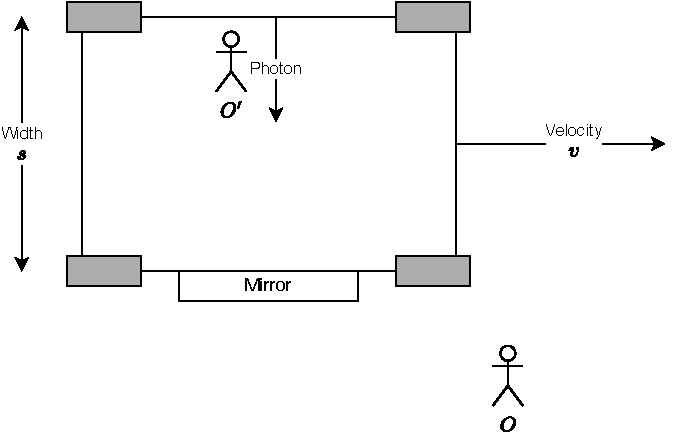
\includegraphics[width=0.7\linewidth]{figures/RelativityDiag1.drawio.pdf}
	\caption{Schematic of a special relativity scenario. The cart, having width $s$, is moving at velocity $v$. On the cart is a co-moving observer ($O'$), and, stationary relative to the cart, is a lab-frame observer ($O$). A photon is propelled from one end of the cart to the other.}
	\label{fig:relativitydiag1}
\end{figure}

The two observers measure the time it takes for the photon to bounce of the mirror and return to its source. The path the photon takes is shown in Figure \ref{fig:relativitydiag1b}.
\begin{figure}[H]
	\centering
	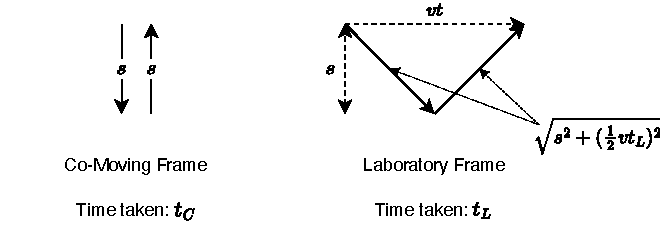
\includegraphics[width=0.7\linewidth]{figures/RelativityDiag1b.drawio.pdf}
	\caption{Schematic of the distances traveled from different frames of reference.}
	\label{fig:relativitydiag1b}
\end{figure}
For $O'$, the time is measured to be $t_C$, however, since the speed of light, $c$ is a constant in any reference frame we can write
\beqn 
c = \frac{2s}{t_C}.
\eeqn 
For $O$, the time is measured to be $t_L$ but the distance traveled by the photon is much greater. Still, $c$ is constant and therefore we write
\beqn 
c = \frac{2\sqrt{s^2 + (\frac{1}{2}vt_L)^2}}{t_L}.
\eeqn 
From the first equation we obtain an expression for $t_C$, i.e.,
\beqn
t_C = \frac{2s}{c},
\eeqn 
and from the second equation we obtain an expression for $t_L$, i.e.,
\beqn 
ct_L &= 2\sqrt{s^2 + (\frac{1}{2}vt_L)^2} \\
\frac{1}{4} c^2 t_L^2 &= s^2 + \frac{1}{4}v^2 t_L^2 \\
\frac{1}{4} t_L^2 (c^2-v^2) &= s^2 \\
t_L^2 &= 4s^2 \frac{1}{c^2 - v^2} \\
\therefore
t_L &= 2s \frac{1}{\sqrt{c^2-v^2}}
\eeqn 

\subsubsection{A useful relation from the clock-readings, e.g. time dilation}
We can deduce several things from these expressions but firstly we define two important items. We define $t'$ as the time passed in the co-moving frame relative to the lab-frame. We also define $t_0$ as the time passed in the lab-frame relative to the co-moving frame. With these defined we can develop expressions for these quantities as follows.

Firstly, time passed in the co-moving frame relative to the lab-frame, $t'$, is simply the ratio of the clock readings $t_C$ to $t_L$, multiplied with an arbitrary time passed in the lab-frame, $t$, i.e.,
\beqn 
t' &= \dfrac{t_C}{t_L} t
= \dfrac{\dfrac{2s}{c}}
{2s\dfrac{1}{\sqrt{c^2-v^2}}} t,
\eeqn 
arriving at
\beqn \label{eq:time_relativity_t_prime}
t' &= \biggr( \sqrt{1-\frac{v^2}{c^2}} \biggr) t.
\eeqn 
Secondly, time passed in the lab-frame relative to the co-moving frame, $t_0$, is simply the opposite ratio $t_L$ to $t_C$, again multiplied with an arbitrary time passed in the lab-frame, $t$, i.e.,
\beqn 
t_0 &= \dfrac{t_L}{t_C} t 
= \dfrac{2s\dfrac{1}{\sqrt{c^2-v^2}}}
{\dfrac{2s}{c}} t
\eeqn 
arriving at
\beqn \label{eq:time_relativity_t0}
t_0 &= \frac{1}{\sqrt{1-\dfrac{v^2}{c^2}}}t.
\eeqn 

These two expressions, i.e., eqs. \eqref{eq:time_relativity_t_prime} and \eqref{eq:time_relativity_t0}, can tell us some interesting things once we plug in some examples for $v$, e.g., for $v=\frac{6}{10} c$, we get $t'=\frac{8}{10}t$ and $t_0=\frac{5}{4}t$. It is easy to see that the clock placed in the co-moving frame runs slow as observed from the lab-frame (i.e. $t'<1$) and the clock placed in the lab-frame runs fast as observed from the co-moving frame (i.e. $t_0>1$). This effect is generally known as \textbf{time dilation}.

Time dilation forms the basis of many other aspects that follow and to that end we define the following,
\beqn
\beta = \frac{v}{c} 
\eeqn
and 
\beqn 
\gamma = \frac{1}{\sqrt{1-\beta^2}}.
\eeqn 
With these definitions our time expresions in eqs. \eqref{eq:time_relativity_t_prime} and \eqref{eq:time_relativity_t0} become
\beqn \label{eq:time_relativity_t_prime2}
t' &= \frac{1}{\gamma} t
\eeqn 
and
\beqn \label{eq:time_relativity_t02}
t_0 &= \gamma t.
\eeqn 


\newpage
\section{Conservation equations}
\subsection{Conservation equation - Radiative transfer}
The basic statement of conservation, is
\beqn 
\frac{1}{c} \frac{\partial I(\position, \Omegabf, \nu, t)}{\partial t} &=
-\Omegabf \dotp \bnabla I(\position, \Omegabf, \nu, t)
- \sigma_t(\position,\nu) I(\position, \Omegabf, \nu, t) \\
&+ \int_0^{\infty} \int_{4\pi} \frac{\nu}{\nu'} \sigma_s(\position,\nu'{\to}\nu,\Omegabf'{\dotp}\Omegabf) I(\position, \Omegabf', \nu', t)  d\nu' d\Omegabf' \\
&+ \sigma_a(\position,\nu) B(\nu,T(\position, t))+S
\eeqn 
where $S$ is any other sources/sinks of radiation intensity. 

\subsection{Radiative transfer assuming isotropic Thompson scattering}
Assuming Thomson-scattering\footnote{Thomson scattering is the elastic scattering of electromagnetic radiation by a free charged particle. The particle's kinetic energy- as well as the photon's frequency, does not change in such a scattering. The scattering is also isotropic.} is the only form of scattering, gives
\beqn 
\frac{1}{c} \frac{\partial I(\position, \Omegabf, \nu, t)}{\partial t} &=
-\Omegabf \dotp \bnabla I(\position, \Omegabf, \nu, t)
- \sigma_t(\position,\nu) I(\position, \Omegabf, \nu, t) \\
&+ \frac{\sigma_s(\position,\nu)}{4\pi} c \RadE(\position, \nu)
+ \sigma_a(\position,\nu) B(\nu,T(\position, t))+S
\eeqn 
where $S$ is any other sources/sinks of radiation intensity. 
\newline
\newline
\textbf{Using energy instead of frequency, $\nu\to E$:}
\beqn 
\frac{1}{c} \frac{\partial I(\position, \Omegabf, E, t)}{\partial t} &=
-\Omegabf \dotp \bnabla I(\position, \Omegabf, E, t)
- \sigma_t(\position,E) I(\position, \Omegabf, E, t) \\
&+ \frac{\sigma_s(\position,E)}{4\pi} c \RadE(\position, E)
+ \sigma_a(\position,E) B(E,T(\position, t))+S
\eeqn 
where $S$ is any other sources/sinks of radiation intensity. 

\subsection{Radiative transfer with material motion corrections}
Applying relativistic corrections for a material in motion, we can derive (e.g., see NUEN 627 lecture 4) the laboratory-frame transport equation
\beqn 
\frac{1}{c} \frac{\partial I(\position, \Omegabf, E, t)}{\partial t} &=
-\Omegabf \dotp \bnabla I(\position, \Omegabf, E, t)
- \biggr(\frac{E_0}{E}\biggr)\sigma_t(\position,E_0) I(\position, \Omegabf, E, t) \\
&+ \biggr(\frac{E}{E_0}\biggr)^2\frac{\sigma_s(\position,E)}{4\pi} \int_{4\pi} \biggr(\frac{E_0}{E'}\biggr) I(\position, \Omegabf', E', t) d\Omegabf'
+ \biggr(\frac{E}{E_0}\biggr)^2 \sigma_a(\position,E_0) B(E_0,T(\position, t))+S,
\eeqn 
where
\beqn 
E_0 = E \gamma \biggr(1-\Omegabf \dotp \frac{\mathbf{u}}{c}\biggr)
\eeqn 
\beqn 
\gamma = \biggr[ 1-\biggr(\dfrac{||\mathbf{u}||}{c}\biggr)^2 \biggr]^{-\frac{1}{2}}
\eeqn 
\beqn 
\frac{E_0}{E'} = \gamma \biggr(1-\Omegabf' \dotp \frac{\mathbf{u}}{c} \biggr)
\eeqn 
\beqn 
E' = E \dfrac{1-\Omegabf \dotp \dfrac{\mathbf{u}}{c}}{1-\Omegabf' \dotp \dfrac{\mathbf{u}}{c}}
\eeqn 

\subsection{Radiative transfer with material velocity dependencies expanded to $\mathcal{O}(v/c)$}
Very ugly derivations in NUEN 627 lecture 5 to get to,
\beqn 
&\frac{1}{c} \frac{\partial I(\position, \Omegabf, E, t)}{\partial t} 
+\Omegabf \dotp \bnabla I(\position, \Omegabf, E, t)
+\sigma_t(\position,E) I(\position, \Omegabf, E, t) \\
=& \frac{\sigma_s(\position,E)}{4\pi} \phi(E)
+ \sigma_a(\position,E) B(E,T(\position, t))\\
&+
\biggr[
\biggr( \sigma_t + E \frac{\partial \sigma_a}{\partial E} \biggr) I
+\frac{\sigma_s}{4\pi}
\biggr(
2\phi - E \frac{\partial \phi}{\partial E}
\biggr)
+2\sigma_a B(E,T)
- B(E,T) E \frac{\partial \sigma_a}{\partial E}
-\sigma_a E \frac{\partial B(E,T)}{\partial E}
\biggr] \Omegabf \dotp \frac{\mathbf{u}}{c} \\
&-\frac{\sigma_s}{4\pi} \biggr( \RadF - E \frac{\partial \RadF}{\partial E} \biggr) \dotp \frac{\mathbf{u}}{c}
\eeqn 
\newline
\newline
\textbf{Voodoo magic Grey Radiation Transport equation:}\newline
Somehow, determined by integrating over energy
\beqn 
\frac{1}{c} \frac{\partial I}{\partial t} 
+\Omegabf \dotp \bnabla I
+\sigma_t(\position) I 
=\frac{\sigma_s}{4\pi} \phi
+ \frac{\sigma_a}{4\pi} a c T^4
-\frac{\sigma_t}{4\pi}  \RadF_0 \dotp \frac{\mathbf{u}}{c} 
+ \frac{\sigma_t}{\pi} \RadE \ \Omegabf \dotp \velocity
\eeqn 
\newline
\newline
\textbf{Radiation energy equation:}\newline 
Obtained by integrating the transport equation over energy and angle
\beqn 
 \frac{\partial \RadE(\position, t)}{\partial t} 
+\bnabla \dotp \RadF(\position, t) &= \int_0^\infty \sigma_a(\position, E) \bigr( 4\pi B(E,T) - \phi(\position, E, t) \bigr) dE \\
&+\int_0^\infty \biggr( \sigma_a + E \frac{\partial \sigma_a}{\partial E} - \sigma_s(E)\biggr)
\RadF \dotp  \frac{\mathbf{u}}{c}
dE
\eeqn 
\newline
\newline 
\textbf{Radiation momentum equation:}\newline
Obtained by first multiplying by $\frac{1}{c} \Omegabf$, then integrating over all directions and energies,
\beqn 
\frac{1}{c^2} \partialderiv{\RadF}{t} + \bnabla \dotp \RadP &= -\int_0^\infty \frac{\sigma_t}{c} \RadF dE \\
&+\int_0^\infty \bigr( \sigma_s \phi + \sigma_a 4\pi B(E,T) \bigr) \frac{\mathbf{u}}{c^2}dE \\
&+\int_0^\infty \biggr( \sigma_a + E \partialderiv{\sigma_a}{E} + \sigma_s\biggr) \RadP \dotp \frac{\mathbf{u}}{c} dE
\eeqn 




\subsection{Grey Radiative Transfer}
\beqn \label{eq:grey_radiative_transfer}
&\frac{1}{c} \frac{\partial I(\position, \Omegabf, t)}{\partial t} 
+\Omegabf \dotp \bnabla I(\position, \Omegabf, t)
+\sigma_t(\position) I(\position, \Omegabf, t) \\
=& \frac{\sigma_s}{4\pi} \phi
+ \frac{\sigma_a}{4\pi} a c T^4\\
&+
\biggr[
\sigma_t  I
+\frac{\sigma_s}{4\pi} 2\phi 
+2\sigma_a \frac{1}{4\pi} acT^4
-\sigma_a E \frac{\partial B(E,T)}{\partial E}
\biggr] \Omegabf \dotp \frac{\mathbf{u}}{c} \\
&-\frac{\sigma_s}{4\pi}  \RadF \dotp \frac{\mathbf{u}}{c}
\eeqn 
\textbf{Radiation energy equation:}\newline 
Obtained by integrating Eq. \eqref{eq:grey_radiative_transfer} over energy and angle
\beqn \label{eq:radiation_energy_equation}
\frac{\partial \RadE(\position, t)}{\partial t} 
+\bnabla \dotp \RadF(\position, t) &=  \sigma_a c \bigr( aT^4 - \RadE \bigr)
+ \bigr( \sigma_a  - \sigma_s\bigr)
\RadF \dotp  \frac{\mathbf{u}}{c} \\
&= \sigma_a c(aT^4 - \RadE_0) - \sigma_t \RadF \dotp \frac{\velocity}{c} 
\eeqn 
\newline
\newline 
\textbf{Radiation momentum equation:}\newline
Obtained by first multiplying Eq. \eqref{eq:grey_radiative_transfer} by $\frac{1}{c} \Omegabf$, then integrating over all directions and energies,
\beqn \label{eq:radiation_momentum_equation}
\frac{1}{c^2} \partialderiv{\RadF}{t} + \bnabla \dotp \RadP &= - \frac{\sigma_t}{c} \RadF  
+ \bigr( \sigma_s c\RadE + \sigma_a acT^4 \bigr) \frac{\mathbf{u}}{c^2} 
+\sigma_t \RadP \dotp \frac{\mathbf{u}}{c} \\
&=  - \frac{\sigma_t}{c} \RadF + \bigr((\sigma_a +\sigma_s -\sigma_a)\RadE + \sigma_a a  T^4\bigr)\frac{\velocity}{c} + \sigma_t \RadP \dotp \frac{\mathbf{u}}{c} \\
&= \frac{1}{c}\biggr[  
- \sigma_t \RadF + \bigr((\sigma_t -\sigma_a)\RadE + \sigma_a a  T^4\bigr)\velocity + \sigma_t \RadP \dotp \velocity 
\biggr]\\
&= -\frac{1}{c}\biggr[  
 \sigma_t \RadF - \bigr((\sigma_t -\sigma_a)\RadE + \sigma_a a  T^4\bigr)\velocity -\sigma_t \RadP \dotp \velocity 
\biggr]\\
\frac{1}{c^2} \partialderiv{\RadF}{t} + \bnabla \dotp \RadP &= -\frac{\sigma_t}{c}
\RadF_0 +  \sigma_a c\bigr(a  T^4 - \RadE \bigr)\frac{\velocity  }{c^2}
\eeqn 

\subsection{Grey Diffusion Approximation}
Approximating the angular dependence of $I(\Omegabf)$ with a $P_1$ spherical harmonic expansion, such that the entries of $\RadP$ are given by
\beqn 
(\RadP)_{i,j}= \frac{1}{3} \RadE \delta_{i,j},
\eeqn 
the radiation energy equation is unaffected but the radiation momentum equation changes. We repeat the radiation energy equation below, and the altered radiation moment equations:
\beqn 
\frac{\partial \RadE}{\partial t} 
+\bnabla \dotp \RadF(\position, t) &=  \sigma_a c \bigr( aT^4 - \RadE \bigr)
+ \bigr( \sigma_a  - \sigma_s\bigr)
\RadF \dotp  \frac{\mathbf{u}}{c},
\eeqn 
\beqn 
\frac{1}{3} \bnabla \RadE = - \frac{\sigma_t}{c} \RadF  
+ \bigr( \sigma_s c\RadE + \sigma_a acT^4 \bigr) \frac{\mathbf{u}}{c^2} 
+\sigma_t \frac{1}{3} \RadE \frac{\mathbf{u}}{c}.
\eeqn 
\newline
\newline 
\textbf{Useful transformations:}\newline 
\begin{subequations}
\beqn 
\RadE_0 = \RadE - \frac{2}{c^2} \RadF \dotp \mathbf{u}
\eeqn 
\beqn 
\RadE = \RadE_0 + \frac{2}{c^2} \RadF_0 \dotp \mathbf{u}
\eeqn 
\beqn \label{eq:F_0_raw}
\RadF_0 = \RadF - \bigr( \RadE \mathbf{u} + \RadP \dotp \mathbf{u} \bigr)
\eeqn 
\beqn 
\RadF = \RadF_0 + \bigr( \RadE_0 \mathbf{u} + \RadP_0 \dotp \mathbf{u} \bigr)
\eeqn 
\beqn 
\RadP_0 = \RadP - \frac{2}{c^2} \mathbf{u} \otimes \RadF
\eeqn 
\beqn 
\RadP = \RadP_0 + \frac{2}{c^2} \mathbf{u} \otimes \RadF_0
\eeqn 
With the $P_1$ approximation
\beqn \label{eq:F0_semi_raw}
\RadF_0 = \RadF - \frac{4}{3} \RadE \mathbf{u}
\eeqn 
\beqn \label{eq:F_semi_raw}
\RadF = \RadF_0 + \frac{4}{3} \RadE \mathbf{u}
\eeqn 
\end{subequations}
Applying these transformations the radiation energy- and moment equation can be expressed as
\beqn 
\frac{\partial \RadE}{\partial t} 
+\bnabla \dotp \RadF(\position, t) &=  \sigma_a c \bigr( aT^4 - \RadE_0 \bigr)
-\sigma_t \RadF \dotp  \frac{\mathbf{u}}{c},
\eeqn 
\beqn 
\frac{1}{3} \bnabla \RadE = - \frac{\sigma_t}{c} \RadF_0
+ \sigma_a c\bigr( aT^4 - \RadE \bigr) \frac{\mathbf{u}}{c^2}.
\eeqn 
Several simplifications to these equations are made. Firstly arriving at the expression for the radiation energy equation,
\beqn 
\frac{\partial \RadE}{\partial t} 
+\bnabla \dotp \RadF(\position, t) &=  \sigma_a c \bigr( aT^4 - \RadE \bigr)
-\sigma_t \RadF_0 \dotp  \frac{\mathbf{u}}{c},
\eeqn 
then the radiation momentum equation,
\beqn 
\frac{1}{3} \bnabla \RadE &= - \frac{\sigma_t}{c} \RadF_0 
\eeqn 
from which we can get expression for $\RadF_0$ and $\RadF$ in terms of $\RadE$ as
\beqn 
\RadF_0 &= -\frac{c}{3\sigma_t} \bnabla \RadE \\
\eeqn 
and
\beqn 
\frac{1}{3} \bnabla \RadE &= - \frac{\sigma_t}{c} \biggr (\RadF - \frac{4}{3} \RadE \mathbf{u} \biggr) \\
\therefore
 \RadF  &= -\frac{c}{3\sigma_t} \bnabla \RadE + \frac{4}{3} \RadE \mathbf{u}.
\eeqn 
These expressions for $\RadF_0$ and $\RadF$ are both then inserted into the radiation energy equation as follows
\beqn 
\frac{\partial \RadE}{\partial t} 
+\bnabla \dotp \RadF(\position, t) &=  \sigma_a c \bigr( aT^4 - \RadE \bigr)
-\sigma_t \RadF_0 \dotp  \frac{\mathbf{u}}{c}
\\
\to
\frac{\partial \RadE}{\partial t} 
+\bnabla \dotp \biggr(  -\frac{c}{3\sigma_t} \bnabla \RadE + \frac{4}{3} \RadE \mathbf{u}  \biggr)
&=  \sigma_a c \bigr( aT^4 - \RadE \bigr)
-\sigma_t \biggr( -\frac{c}{3\sigma_t} \bnabla \RadE \biggr) \dotp  \frac{\mathbf{u}}{c} 
\\
\to 
\frac{\partial \RadE}{\partial t} 
+\bnabla \dotp \biggr(  -\frac{c}{3\sigma_t} \bnabla \RadE \biggr) + \frac{4}{3} \bnabla  \dotp \bigr( \RadE \mathbf{u}  \bigr)
&=  \sigma_a c \bigr( aT^4 - \RadE \bigr)
+\frac{1}{3} \bnabla \RadE  \dotp  \velocity.
\eeqn 

Arriving at a \textbf{diffusion form} of the \textbf{radiation energy equation},
\beqn 
\frac{\partial \RadE}{\partial t} 
+\bnabla \dotp \biggr(  -\frac{c}{3\sigma_t} \bnabla \RadE \biggr) + \frac{4}{3} \bnabla \dotp \bigr( \RadE \mathbf{u}  \bigr)
&=  \sigma_a c \bigr( aT^4 - \RadE \bigr)
+\frac{1}{3} \bnabla \RadE  \dotp  \velocity.
\eeqn

\vspace{1cm}
\subsection{Conservation equation for fluid flow}
The governing equations we consider here are the Euler equations defined as
\beqn 
\partialderiv{\rho}{t} + \bnabla \dotp (\rho \velocity) = 0
\eeqn 
\beqn 
\partialderiv{(\rho\velocity)}{t} + \bnabla \dotp \{ \rho \velocity \otimes \velocity\}  + \bnabla p = \mathbf{f},
\eeqn 
\beqn 
\partialderiv{E}{t} + \bnabla \dotp [(E + p)\velocity] = q
\eeqn 
where $\rho$ is the fluid density, $\velocity = [u_x, u_y, u_z] =[u,v,w]$ is the fluid velocity in cartesian coordinates, $p$ is the fluid pressure, $E$ is the material energy-density comprising kinetic energy-density, $\frac{1}{2} \rho ||\velocity||^2$, and internal energy-density, $\rho e$, such that $E = \frac{1}{2} \rho ||\velocity||^2 + \rho e$, where $e$ is the specific internal energy. The values $q$ and $\mathbf{f}$ are abstractly used here as energy- and moment- sources/sinks, respectively.

The ideal gas law provides the closure relation
\beqn 
p = (\gamma - 1) \rho e
\eeqn 
where $\gamma$ is the ratio of the constant-pressure specific heat, $c_p$, to the constant-volume specific heat, $c_v$, i.e., $\gamma = \frac{c_p}{c_v}$, and is a material property.
\newline
\newline
\textbf{Coupling terms:}\newline
\beqn 
\mathbf{f} &= \frac{\sigma_t}{c} \RadF_0 \\ &= -\frac{1}{3} \bnabla \RadE
\eeqn 
and
\beqn 
q &= - \biggr(\sigma_a c (a T^4 - \RadE) - \sigma_t \RadF_0 \dotp \frac{\mathbf{u}}{c} \biggr)\\
&= \sigma_a c (\RadE - a T^4) - \frac{1}{3} \bnabla \RadE \dotp \velocity
\eeqn 

\newpage
\section{Solver A - Radiation Hydrodynamics Grey Diffusion}
The set of Radiation Hydrodynamics Grey Diffusion Equations are
\begin{subequations}
\beqn 
\partialderiv{\rho}{t} + \bnabla \dotp (\rho \velocity) = 0
\eeqn 
\beqn 
\partialderiv{(\rho\velocity)}{t} + \bnabla \dotp \{ \rho \velocity \otimes \velocity\}  + \bnabla p 
= -\frac{1}{3} \bnabla \RadE,
\eeqn 
\beqn 
\partialderiv{E}{t} + \bnabla \dotp [(E + p)\velocity] 
= \sigma_a c (\RadE - a T^4) - \frac{1}{3} \bnabla \RadE \dotp \velocity
\eeqn 
\beqn 
\frac{\partial \RadE}{\partial t} 
+\bnabla \dotp \biggr(  -\frac{c}{3\sigma_t} \bnabla \RadE \biggr) + \frac{4}{3} \bnabla \bigr( \RadE \mathbf{u}  \bigr)
&=  \sigma_a c \bigr( aT^4 - \RadE \bigr)
+\frac{1}{3} \bnabla \RadE  \dotp \velocity.
\eeqn
where
\beqn 
E = \frac{1}{2} \rho ||\velocity||^2 + \rho e,
\eeqn 
\beqn 
p = (\gamma - 1) \rho e,
\eeqn 
\beqn 
T = \frac{1}{C_v} e
\eeqn 
\beqn 
\sigma_t(T) &= \sigma_s(T) + \sigma_a(T)\\
\eeqn 
\beqn 
\sigma_s(T) &= \rho \kappa_s (T) \\
\eeqn 
\beqn 
\sigma_a(T) &= \rho \kappa_a (T)
\eeqn 
\end{subequations}



\subsection{Definitions}
First we define the following terms
\begin{subequations}
\begin{itemize}
\item The radiation emission and absorption, the radiation momentum source, and the radiation energy source
\beqn 
S_{ea} =  \sigma_a c \bigr( aT^4 - \RadE \bigr)
%\quad \quad \quad
\eeqn 
\beqn 
\mathbf{S}_{rp} = \frac{1}{3} \bnabla \RadE
\eeqn 
\beqn 
S_{re} =S_{ea} 
+\frac{1}{3} \bnabla \RadE  \dotp \velocity
\eeqn 
\item The conserved hydrodynamic variables, $\HydroU$, and associated hydrodynamic flux, $\HydroF$,
\beqn
\HydroU = 
\begin{bmatrix}
	\rho \\ \rho \mathbf{u} \\ E
\end{bmatrix} 
\quad \quad
\HydroF = 
\begin{bmatrix}
	\rho u \\
	\rho uu + p \\
	\rho u v \\
	\rho u w \\
	(E+p)u
\end{bmatrix}
\eeqn 
\item The stationary reference frame radiation energy flux
\beqn 
\RadJ = -\frac{c}{3\sigma_t} \bnabla \RadE
\eeqn 
\end{itemize}
\end{subequations}

\noindent
Next, we use these terms to define a more condensed version of the RHGD equations. 
\beqn 
\partialderiv{\HydroU}{t} + \bnabla \dotp \HydroF(\HydroU) = 
\begin{bmatrix}
	0 \\
-\mathbf{S}_{rp} \\
-S_{re} 
\end{bmatrix}
\eeqn 
\beqn 
\frac{\partial \RadE}{\partial t} 
+\bnabla \dotp \RadJ  + \frac{4}{3} \bnabla \dotp \bigr( \RadE \mathbf{u}  \bigr)
&=  S_{ea} + \frac{1}{3} \bnabla \RadE  \dotp \velocity.
\eeqn

\newpage
\subsection{Finite Volume Spatial Discretization}
To apply a finite volume spatial discretization we integrate our time-discretized equations over the volume, $V_c$, of cell $c$, and afterwards divide by $V_c$. This leaves all the terms containing $\tau$ unchanged. In this process we develop the following terms:

\subsubsection{Hydrodynamic and Radiation-energy advection}
\label{section:fv_hydro_and_radE_advection}
\beqn 
\frac{1}{V_c} \int_{V_c} 
\bnabla \dotp \HydroF (\HydroU) 
dV = \frac{1}{V_c}
\sum_f \AreaVec_f \dotp  \HydroF(\HydroU_f)
\eeqn 

\beqn 
\frac{1}{V_c} \int_{V_c} 
\biggr(\frac{4}{3} \bnabla \dotp \bigr(\RadE \velocity)\biggr)
dV = \frac{1}{V_c}
\sum_f \frac{4}{3}  \AreaVec_f \dotp (\RadE \velocity)_f
\eeqn 
The face values are reconstructed from gradients in both the predictor and corrector phases. In the corrector-phase the hydrodynamic flux, $\HydroF$, is used in its earlier defined form, whilst in the corrector-phase the flux is determined by an approximate Riemann-solver, i.e., the HLLC Riemann solver.
\newline
\newline 
\textbf{Predictor phases:}\newline 
For the predictor phase we have the following:
\beqn 
\bnabla \dotp \HydroF (\HydroU)
\mapsto 
\frac{1}{V_c}
\sum_f \AreaVec_f \dotp  \HydroF(\HydroU_f)
\eeqn 
\beqn 
\biggr(\frac{4}{3} \bnabla \dotp \bigr(\RadE \velocity)\biggr)
\mapsto 
\frac{1}{V_c}
\sum_f \frac{4}{3}  \AreaVec_f \dotp (\RadE \velocity)_f
\eeqn 

\beqn 
\HydroU_f = \HydroU_c + (\position_f - \position_c) \dotp \{ \bnabla\HydroU \}_c
\eeqn 
\beqn 
\RadE_f = \RadE_c + (\position_f - \position_c) \dotp \{ \bnabla\RadE \}_c
\eeqn 

\noindent
\textbf{Corrector phases:}\newline
For the corrector phase we have the following:
\beqn 
\bnabla \dotp \HydroF (\HydroU)
\mapsto 
\frac{1}{V_c}
\sum_f \AreaVec_f \dotp  \mathbf{F}^{*hllc}(\HydroU_f)
\eeqn 
\beqn 
\biggr(\frac{4}{3} \bnabla \dotp \bigr(\RadE \velocity)\biggr)
\mapsto 
\frac{1}{V_c}
\sum_f \frac{4}{3}  \AreaVec_f \dotp (\RadE \velocity)_{upw}
\eeqn 
where
\beqn 
\HydroU_f = \HydroU_c+ (\position_f - \position_c) \dotp \{ \bnabla\HydroU \}_c
\eeqn  
\beqn
(\RadE \velocity)_{upw} =
\begin{cases}
	(\RadE \velocity)_{c,f} , &\text{ if } 
	\velocity_{c,f} \dotp  \NormalVec_f > 0 \text{ and } \velocity_{cn,f} \dotp  \NormalVec_f > 0 
	\quad  \rightarrow | \rightarrow \\
	(\RadE \velocity)_{cn,f} , &\text{ if } 
	\velocity_{c,f} \dotp  \NormalVec_f < 0 \text{ and } \velocity_{cn,f} \dotp  \NormalVec_f < 0
	\quad  \leftarrow | \leftarrow \\
	(\RadE \velocity)_{cn,f} + (\RadE \velocity)_{c,f}, &\text{ if } 
	\velocity_{c,f} \dotp  \NormalVec_f > 0 \text{ and } \velocity_{cn,f} \dotp  \NormalVec_f < 0 
	\quad  \rightarrow | \leftarrow \\
	0, &\text{ if } 
	\velocity_{c,f} \dotp  \NormalVec_f < 0 \text{ and } \velocity_{cn,f} \dotp  \NormalVec_f > 0
	\quad  \leftarrow | \rightarrow \\
\end{cases}
\eeqn 
\beqn 
\RadE_{c,f} = \RadE_c + (\position_f - \position_c) \dotp \{ \bnabla\RadE \}_c
\eeqn

\newpage
\subsubsection{Density and momentum updates} 
\label{section:fv_density_momentum_update}
We apply the same process as before:
\beqn 
-\frac{1}{V_c} \int_{V_c} \mathbf{S}_{rp} dV = -\frac{1}{V_c}  \sum_f \frac{1}{3} \AreaVec_f \RadE_f,
\eeqn 
however, here we want $\RadE_f$ to satisfy the following relationship
\beqn 
\frac{D_c}{||\position_{cf}||} (\RadE_f - \RadE_c) = 
\frac{D_{cn}}{||\position_{fcn}||} (\RadE_{cn} - \RadE_f) 
\eeqn 
where
\beqn 
D_c = -\frac{c}{3\sigma_{t,c}}
\eeqn 
and where $\position_{cf}$ is the vector from cell $c$'s centroid to the face centroid, $\position_{fcn}$ is the vector from the face centroid to cell $cn$'s centroid (where cell $cn$ is the neighbor to $c$ at face $f$). The norm $||\dotp||$ refers to the $L_2$ norm.

Solving the above relationship for $\RadE_f$ we first set
\beq 
k_c = \frac{D_c}{||\position_{cf}||} , \quad \quad
k_{cn} = \frac{D_{cn}}{||\position_{fcn}||}
\eeq 
then get
\beqn 
k_c \RadE_f - k_c \RadE_c &= k_{cn}  \RadE_{cn} - k_{cn}  \RadE_f \\
\to \quad 
(k_c + k_{cn} ) \RadE_f &= k_{cn}  \RadE_{cn} + k_c \RadE_c \\
\therefore
\RadE_f &= \frac{k_{cn}  \RadE_{cn} + k_c \RadE_c}{k_c +k_{cn} } .
\eeqn 
\newline
\newline 
\textbf{Predictor and corrector phases:} \newline 
We do the same for both,
\beqn
-\mathbf{S}_{rp} \mapsto  -\frac{1}{V_c}  \sum_f  \frac{1}{3} \AreaVec_f \RadE_f
\eeqn



\subsubsection{Energy equations}
\label{section:fv_energy_equations}
Only two terms require special consideration here. They are: the divergence of the co-moving frame radiation energy flux, and the kinetic energy terms source terms,
\beqn 
\frac{1}{V_c} \int_{V_c} \bnabla \dotp \RadJ \ dV &= \frac{1}{V_c} \sum_f \AreaVec_f \dotp (\RadJ)_f \\
\frac{1}{V_c} \int_{V_c} \frac{1}{3} \bnabla \RadE \dotp \velocity \ dV &= \frac{1}{V_c} \sum_f \frac{1}{3} \AreaVec_f \dotp (\RadE \velocity)_f.
\eeqn 

\paragraph{The diffusion term} \mbox{}\\
Considering the $\RadJ$-term first, we apply Gauss' divergence theorem to get
\beqn 
\bnabla \dotp \RadJ \mapsto \frac{1}{V_c} \sum_f \AreaVec_f \dotp (\RadJ)_f.
\eeqn 
For $(\RadJ)_f$ we have
\beqn 
(\RadJ)_f = - \frac{c}{3\sigma_{tf}} \bigr(\bnabla \RadE \bigr)_f.
\eeqn 
Now define
\beqn
D_f &= - \frac{c}{3\sigma_{tf}}.
\eeqn 
To find $D_f$ we seek the equivalence:
\beqn
D_f \frac{\RadE_{cn} - \RadE_c}{|| \position_{cn} - \position_{c} ||} 
=
D_c \frac{\RadE_{f} - \RadE_c}{|| \position_{f} - \position_{c} ||} 
=
D_{cn} \frac{\RadE_{cn} - \RadE_f}{|| \position_{cn} - \position_{f} ||} 
\eeqn
Now let us define
\beqn 
k_c &= \frac{D_c}{|| \position_{f} - \position_{c} ||} \\
k_{cn} &= \frac{D_{cn}}{|| \position_{cn} - \position_{f} ||} \\
\eeqn 
Now
\beqn
k_c (\RadE_f - \RadE_c) &= k_{cn} (\RadE_{cn} - \RadE_f) \\
 (k_c +k_{cn}) \RadE_f &= k_{cn} \RadE_{cn} + k_c \RadE_{c} \\
 \therefore
 \RadE_f &= \frac{k_{cn} \RadE_{cn} + k_c \RadE_{c}}{k_c + k_{cn}}
\eeqn
Now we choose any of the right-two terms in the three way equality and plug the expression for $\RadE_f$,
\beqn 
&\quad k_c (\RadE_f - \RadE_c) \\
&= k_c \biggr(
\frac{k_{cn} \RadE_{cn} + k_c \RadE_{c}}{k_c + k_{cn}} - \RadE_c
\biggr) \\
&= k_c \biggr(
\frac{k_{cn} \RadE_{cn} + k_c \RadE_{c} - k_c\RadE_c -k_{cn} \RadE_c}{k_c + k_{cn}}
\biggr) \\
\therefore 
D_f \frac{\RadE_{cn} - \RadE_c}{|| \position_{cn} - \position_{c} ||} 
&= \frac{k_c k_{cn}}{k_c + k_{cn}} \bigr(\RadE_{cn} - \RadE_c \bigr)\\
\therefore
D_f &= \frac{k_c k_{cn}}{k_c + k_{cn}}  || \position_{cn} - \position_{c} ||
\eeqn 
From the earlier expression for $(\RadF_0)_f$, we can write
\beqn 
(\RadJ)_f = D_f \bigr( \RadE_{cn} - \RadE_c \bigr) \frac{\position_{cn} - \position_{c}}{|| \position_{cn} - \position_{c}||^2}
\eeqn 
for which we can define
\beqn 
\mathbf{k}_f = D_f  \frac{\position_{cn} - \position_{c}}{|| \position_{cn} - \position_{c}||^2}
\eeqn 
such that we finally arrive at
\beqn 
(\RadJ)_f = \mathbf{k}_f \bigr( \RadE_{cn} - \RadE_c \bigr).
\eeqn 


\paragraph{The kinetic energy term} \mbox{} \\
For the kinetic energy source terms, we similarly have
\beqn 
\biggr( \frac{1}{3} \bnabla \RadE \dotp \velocity \biggr)^n
\mapsto 
\frac{1}{V_c} \sum_f \frac{1}{3} \AreaVec_f \dotp (\RadE_f^n \velocity_f^n)
\eeqn 
where we use the reconstructed values as in the Hydrodynamic and radiation-energy advection portion.

\newpage
\subsection{Temporal scheme - Implicit Euler Predictor, Crank-Nicolson Corrector}
\begin{subequations}
\beqn 
\partialderiv{\HydroU}{t} + \bnabla \dotp \HydroF(\HydroU) = 
\begin{bmatrix}
	0 \\
	-\mathbf{S}_{rp} \\
	-S_{re} 
\end{bmatrix}
\eeqn 
\beqn 
\frac{\partial \RadE}{\partial t} 
+\bnabla \dotp \RadJ  + \frac{4}{3} \bnabla \dotp \bigr( \RadE \mathbf{u}  \bigr)
&=  S_{re}.
\eeqn
\end{subequations}



\subsubsection{Predictor phase}
$\tau = \dfrac{1}{\half \Delta t}$
\begin{subequations}
	\beqn 
	\tau (\HydroU^{n*} - \HydroU^{n}) + \bnabla \dotp \HydroF(\HydroU^{n}) = \mathbf{0}
	\eeqn 
	
	\beqn 
	\tau \begin{pmatrix}
		\HydroRhoRhoU^{n+\half} - \HydroRhoRhoU^{n*}
	\end{pmatrix} =  
	\begin{bmatrix}
		0 \\
		-\frac{1}{3} \bnabla \RadE
	\end{bmatrix}^{n}
	\eeqn 
	
	\beqn 
	\tau (\RadE^{n*} - \RadE^{n}) + \biggr(\frac{4}{3} \bnabla \dotp \bigr(\RadE \velocity)\biggr)^{n} = 0
	\eeqn 
	
	\beqn 
	\tau (E^{n+\half} - E^{n*}) = 
	-\theta_1 S_{ea}^{n+\half}
	- \theta_2 S_{ea}^n
	- \biggr(\frac{1}{3} \bnabla \RadE \dotp \velocity \biggr)^{n}
	\eeqn 
	
	\beqn 
	\tau (\RadE^{n+\half} - \RadE^{n*}) 
	+  \theta_1 \bnabla \dotp \RadJ^{n+\half} 
	+ \theta_2 \bnabla \dotp \RadJ^{n}= 
	 \theta_1 S_{ea}^{n+\half}
	+ \theta_2 S_{ea}^n
	+ \biggr( \frac{1}{3} \bnabla \RadE \dotp \velocity \biggr)^{n}
	\eeqn
For $S_{ea}$ and $\RadJ$ both at $n+\half$:
	\beqn 
	\sigma^{n+\half} &= \rho^{n+\half}\kappa(T^n)
	\eeqn 
	
	\beqn 
	T^{4,n+\half} = T^{4,n*} + \frac{4T^{3,n*}}{C_v} (e^{n+\half}-e^{n*})
	\eeqn 
	
\end{subequations}

%\newpage
\subsubsection{Corrector phase}
$\tau = \dfrac{1}{\Delta t}$
\begin{subequations}
	\beqn 
	\tau (\HydroU^{n+\half*} - \HydroU^{n}) + \bnabla \dotp \HydroF(\HydroU^{n+\half}) = \mathbf{0}
	\eeqn 
	
	\beqn 
	\tau 
	\begin{pmatrix}
	\HydroRhoRhoU^{n+1} - \HydroRhoRhoU^{n+\half*}
	\end{pmatrix} = 
    \begin{bmatrix}
		0 \\
		-\frac{1}{3} \bnabla \RadE
	\end{bmatrix}^{n+\half}
	\eeqn 
	
	\beqn 
	\tau (\RadE^{n+\half*} - \RadE^{n}) + \biggr(\frac{4}{3} \bnabla \dotp \bigr(\RadE \velocity)\biggr)^{n+\half} = 0
	\eeqn 
	
	\beqn 
	\tau (E^{n+1} - E^{n+\half*}) = 
	-\theta_1 S_{ea}^{n+1}
	- \theta_2 S_{ea}^{n}
	- \biggr(\frac{1}{3} \bnabla \RadE \dotp \velocity \biggr)^{n+\half}
	\eeqn 
	
	\beqn 
	\tau (\RadE^{n+1} - \RadE^{n+\half*}) 
	+ \theta_1 \bnabla \dotp  \RadJ^{n+1} 
	+ \theta_2 \bnabla \dotp \RadJ^{n} = 
	\theta_1 S_{ea}^{n+1}
	+\theta_2 S_{re}^{n}
	+ \biggr( \frac{1}{3} \bnabla \RadE \dotp \velocity \biggr)^{n+\half}
	\eeqn
For $S_{ea}$ and $\RadJ$ both at $n+1$:
	\beqn 
	\sigma^{n+1} &= \rho^{n+1}\kappa(T^{n+\half})
	\eeqn 
	
	\beqn 
	T^{4,n+1} = T^{4,n+\half*} + \frac{4T^{3,n+\half*}}{C_v} (e^{n+1}-e^{n+\half*})
	\eeqn 
	

\end{subequations}






\newpage
\subsubsection{General energy equations, Predictor and Corrector phase, with $\theta$ factors}
Time integration scheme A uses \textbf{implicit Euler} for the predictor phase and \textbf{Crank-Nicolson} in the corrector phase. Both these schemes can be represented wit a general $\theta$-scheme where we define:
\beqn
\theta_1 &\in [0,1] \\
\theta_2 &= 1-\theta_1.
\eeqn
\noindent
For implicit Euler, $\theta_1 = 1, \ \theta_2=0$, and for Crank-Nicolson, $\theta_1 = \theta_2 = \half$. With these factors defined we can repeat the energy equations and apply a series of manipulations. First we attempt to segregate known terms from all unknown terms. Thereafter we eliminate the internal energy, $e$, from the two sets of equations to get a single formulation for the radiation energy, $\RadE$. The latter formulation forms a diffusion system that needs to be assembled and solved for $\RadE$.


\begin{subequations}
	\beqn 
	\tau (E^{n+1} - E^{n+\half*}) = 
	-\theta_1 \sigma_a^{n+1} c  \biggr( 
	a T^{4,n+1}   -\RadE^{n+1} 
	\biggr)
	- \theta_2 S_{ea}^{n}
	- \biggr(\frac{1}{3} \bnabla \RadE \dotp \velocity \biggr)^{n+\half}
	\eeqn 
	
	\beqn 
	\tau (\RadE^{n+1} - \RadE^{n+\half*}) 
	+  \bnabla \dotp \bigr( \theta_1 \RadJ^{n+1} +  \theta_2 \RadJ^{n} \bigr)= 
	\theta_1 \sigma_a^{n+1} c \biggr( 
	a T^{4,n+1}   -\RadE^{n+1} 
	\biggr)
	+\theta_2 S_{re}^{n}
	+ \biggr( \frac{1}{3} \bnabla \RadE \dotp \velocity \biggr)^{n+\half}
	\eeqn
	
	
	\beqn 
	T^{4,n+1} = T^{4,n+\half*} + \frac{4T^{3,n+\half*}}{C_v} (e^{n+1}-e^{n+\half*})
	\eeqn 

\splitline
\end{subequations}

Define:
\beqn 
k_1 &= \theta_1 \sigma_a^{n+1} c \\
k_2 &= \frac{4 T^{3,n+\half*}}{C_v}
\eeqn 
\splitline

and plug them into the equations above,
\begin{subequations}
	\beqn 
	\tau (E^{n+1} - E^{n+\half*}) = 
	-k_1  \biggr( 
	a T^{4,n+1}   -\RadE^{n+1} 
	\biggr)
	- \theta_2 S_{ea}^{n}
	- \biggr(\frac{1}{3} \bnabla \RadE \dotp \velocity \biggr)^{n+\half}
	\eeqn 
	
	\beqn 
	\tau (\RadE^{n+1} - \RadE^{n+\half*}) 
	+ \bnabla \dotp \bigr( \theta_1 \RadJ^{n+1} +  \theta_2 \RadJ^{n} \bigr)= 
	k_1 \biggr( 
	a T^{4,n+1}   -\RadE^{n+1} 
	\biggr)
	+\theta_2 S_{re}^{n}
	+ \biggr( \frac{1}{3} \bnabla \RadE \dotp \velocity \biggr)^{n+\half}
	\eeqn
	
	
	\beqn 
	T^{4,n+1} = T^{4,n+\half*} + k_2 (e^{n+1}-e^{n+\half*})
	\eeqn 
\end{subequations}

\splitline

ungroup right-hand side elements by multiplying out terms within parentheses,
\begin{subequations}
	\beqn 
	\tau (E^{n+1} - E^{n+\half*}) = 
	-k_1  a T^{4,n+1}   + k_1 \RadE^{n+1} 
	- \theta_2 S_{ea}^{n}
	- \biggr(\frac{1}{3} \bnabla \RadE \dotp \velocity \biggr)^{n+\half}
	\eeqn 
	
	\beqn 
	\tau (\RadE^{n+1} - \RadE^{n+\half*}) 
	+ \bnabla \dotp \bigr( \theta_1 \RadJ^{n+1} + \theta_2 \RadJ^{n} \bigr)= 
	k_1 a T^{4,n+1}   -k_1\RadE^{n+1} 
	+\theta_2 S_{re}^{n}
	+ \biggr( \frac{1}{3} \bnabla \RadE \dotp \velocity \biggr)^{n+\half}
	\eeqn
	
	
	\beqn 
	T^{4,n+1} = T^{4,n+\half*} + k_2 (e^{n+1}-e^{n+\half*})
	\eeqn 
\end{subequations}

\splitline

now plug in the temperature equation into both the energy equations,
\begin{subequations}
	\beqn 
	\tau (E^{n+1} - E^{n+\half*}) = 
	-k_1  a \big(T^{4,n+\half*} + k_2 (e^{n+1}-e^{n+\half*})\big)   + k_1 \RadE^{n+1} 
	- \theta_2 S_{ea}^{n}
	- \biggr(\frac{1}{3} \bnabla \RadE \dotp \velocity \biggr)^{n+\half}
	\eeqn 
	
	\beqn 
	\tau (\RadE^{n+1} - \RadE^{n+\half*}) 
	+ \bnabla \dotp \bigr( \theta_1 \RadJ^{n+1} + \theta_2 \RadJ^{n} \bigr)= 
	k_1 a \big(T^{4,n+\half*} + k_2 (e^{n+1}-e^{n+\half*})\big)   -k_1\RadE^{n+1} 
	+\theta_2 S_{re}^{n}
	+ \biggr( \frac{1}{3} \bnabla \RadE \dotp \velocity \biggr)^{n+\half}
	\eeqn
\end{subequations}

\splitline

ungroup elements on the both the right-hand sides,
\begin{subequations}
	\beqn 
	\tau (E^{n+1} - E^{n+\half*}) = 
	-k_1  a T^{4,n+\half*} -k_1  a k_2 e^{n+1} + k_1  a k_2 e^{n+\half*}
	+ k_1 \RadE^{n+1} 
	- \theta_2 S_{ea}^{n}
	- \biggr(\frac{1}{3} \bnabla \RadE \dotp \velocity \biggr)^{n+\half}
	\eeqn 
	
	\beqn 
	\tau (\RadE^{n+1} - \RadE^{n+\half*}) 
	+ \bnabla \dotp \bigr( \theta_1 \RadJ^{n+1} + \theta_2 \RadJ^{n} \bigr)= 
	k_1 a T^{4,n+\half*} + k_1 a k_2 e^{n+1} - k_1 a k_2 e^{n+\half*}
	-k_1\RadE^{n+1} 
	+\theta_2 S_{re}^{n}
	+ \biggr( \frac{1}{3} \bnabla \RadE \dotp \velocity \biggr)^{n+\half}
	\eeqn
\end{subequations}

\splitline

Define:
\beqn 
k_3 &= -k_1  a T^{4,n+\half*} + k_1  a k_2 e^{n+\half*}
- \theta_2 S_{ea}^{n}
- \biggr(\frac{1}{3} \bnabla \RadE \dotp \velocity \biggr)^{n+\half} \\
k_4 &= -k_1 a k_2
\eeqn 

\splitline

and plug them into the equations above,
\begin{subequations}
	\beqn 
	\tau (E^{n+1} - E^{n+\half*}) = 
	k_4 e^{n+1} 
	+ k_1 \RadE^{n+1} 
	+ k_3
	\eeqn 
	
	\beqn 
	\tau (\RadE^{n+1} - \RadE^{n+\half*}) 
	+ \bnabla \dotp \bigr( \theta_1 \RadJ^{n+1} + \theta_2 \RadJ^{n} \bigr)= 
	-k_4 e^{n+1} 
	-k_1\RadE^{n+1} 
	-k_3
	\eeqn
\end{subequations}

\splitline

Note:
\beqn
E^{n+1} = ( \half \rho ||\velocity||^2 )^{n+1} 
+ \rho^{n+1} e^{n+1}
\eeqn 

\splitline

which gives,
\begin{subequations}
	\beqn 
	\tau \big( ( \half \rho ||\velocity||^2 )^{n+1} 
	+ \rho^{n+1} e^{n+1} - E^{n+\half*}\big) = 
	k_4 e^{n+1} 
	+ k_1 \RadE^{n+1} 
	+ k_3
	\eeqn 
	
	\beqn 
	\tau (\RadE^{n+1} - \RadE^{n+\half*}) 
	+ \bnabla \dotp \bigr( \theta_1 \RadJ^{n+1} + \theta_2 \RadJ^{n} \bigr)= 
	-k_4 e^{n+1} 
	-k_1\RadE^{n+1} 
	-k_3
	\eeqn
\end{subequations}

\splitline

ungroup the material energy in the first equation,
\begin{subequations}
	\beqn 
	\tau ( \half \rho ||\velocity||^2 )^{n+1} 
	+ \tau \rho^{n+1} e^{n+1} - \tau E^{n+\half*} = 
	k_4 e^{n+1} 
	+ k_1 \RadE^{n+1} 
	+ k_3
	\eeqn 
	
	\beqn 
	\tau (\RadE^{n+1} - \RadE^{n+\half*}) 
	+ \theta_1 \bnabla \dotp  \RadJ^{n+1} + \theta_2 \bnabla \dotp \RadJ^{n} = 
	-k_4 e^{n+1} 
	-k_1\RadE^{n+1} 
	-k_3
	\eeqn
\end{subequations}

\splitline

and isolate the internal energy in the first equation,
\begin{subequations}
	\beqn 
	(\tau \rho^{n+1}  - k_4 )e^{n+1} = 
	k_1 \RadE^{n+1} 
	+ k_3 -\tau ( \half \rho ||\velocity||^2 )^{n+1} 
	+ \tau E^{n+\half*} 
	\eeqn 
	
	\beqn 
	\tau (\RadE^{n+1} - \RadE^{n+\half*}) 
	+ \theta_1 \bnabla \dotp  \RadJ^{n+1} + \theta_2 \bnabla \dotp \RadJ^{n} = 
	-k_4 e^{n+1} 
	-k_1\RadE^{n+1} 
	-k_3
	\eeqn
\end{subequations}

\splitline

Define:
\beqn 
k_5 &= \frac{k_1}{\tau \rho^{n+1}  - k_4} \\
k_6 &= \frac{ k_3 -\tau ( \half \rho ||\velocity||^2 )^{n+1} 
	+ \tau E^{n+\half*} }{\tau \rho^{n+1}  - k_4}
\eeqn 

\splitline

and plug these constants into the first equation above,
\begin{subequations}
	\beqn 
	e^{n+1} = 
	k_5 \RadE^{n+1} 
	+ k_6
	\eeqn 
	
	\beqn 
	\tau (\RadE^{n+1} - \RadE^{n+\half*}) 
	+ \theta_1 \bnabla \dotp  \RadJ^{n+1} + \theta_2 \bnabla \dotp \RadJ^{n} = 
	-k_1\RadE^{n+1} 
	-k_3
	-k_4 e^{n+1} 
	\eeqn
\end{subequations}

\splitline

now plug the first equation into the second,
\begin{subequations}
	\beqn 
	\tau (\RadE^{n+1} - \RadE^{n+\half*}) 
	+ \theta_1 \bnabla \dotp  \RadJ^{n+1} + \theta_2 \bnabla \dotp \RadJ^{n} = 
	-k_1\RadE^{n+1} 
	-k_3
	-k_4 k_5 \RadE^{n+1} -k_4 k_6
	\eeqn
\end{subequations}

\splitline

now collect all the $\RadE^{n+1}$ terms on the left-hand side,
\begin{subequations}
	\beqn 
	\big( \tau + k_1 + k_4 k_5\big) \RadE^{n+1} 
	+ \theta_1 \bnabla \dotp  \RadJ^{n+1} = 
	-k_3
	-k_4 k_6
	+ \tau \RadE^{n+\half*}
	- \theta_2 \bnabla \dotp \RadJ^{n}
	\eeqn
\end{subequations}

\splitline 

Recall:
\beqn 
\bnabla \dotp \RadJ \mapsto 
\frac{1}{V_c} \sum_f \AreaVec_f \dotp (\RadJ)_f
\eeqn
and
\beqn 
(\RadJ)_f = \mathbf{k}_f ( \RadE_{cn} - \RadE_c)
\eeqn  

\splitline

which gives the system,
\begin{subequations}
	\beqn 
	\big( \tau + k_1 + k_4 k_5\big) \RadE^{n+1} 
	+ 
	\frac{\theta_1}{V_c} \sum_f \AreaVec_f \dotp  \mathbf{k}_f^{n+1} ( \RadE_{cn}^{n+1} - \RadE_c^{n+1}) 
	= 
	-k_3
	-k_4 k_6
	+ \tau \RadE^{n+\half*}
	- 
	\frac{\theta_2}{V_c} \sum_f \AreaVec_f \dotp  \mathbf{k}_f^{n} ( \RadE_{cn}^{n} - \RadE_c^{n}) 
	\eeqn
\end{subequations}

\splitline

This system is SPD and in one dimension forms a tridiagonal system.





\newpage
\subsubsection{Using the energy related algebra for both the predictor and the corrector}
To perform the energy related algebra for the corrector step we need the following inputs:
\beq
&\kappa_a^n &&\text{For }\sigma_a^n \text{ in }S_{ea}^n \\
&\kappa_t^n &&\text{For }\sigma_t^n \text{ in }\bnabla \dotp \RadJ^{n}\\
&\kappa_a^{n+\half} &&\text{For }\sigma_a^{n+1} \text{ in }S_{ea}^{n+1} \\
&\kappa_t^{n+\half} &&\text{For }\sigma_t^{n+1} \text{ in }\bnabla \dotp \RadJ^{n+1}\\
&C_v && \text{ For the linearization of } T^{4,n+1}\\
&\tau && \text{ For the time constant} \\
&\theta_1 ,\theta_2 &&\text{ For the time scheme} \\
&\HydroU^{n} && \text{ For } T, \rho \text{ in } S_{ea}^n \\
&\HydroU^{n+\half} && \text{ For } \velocity \text{ in }  \biggr( \frac{1}{3} \bnabla \RadE \dotp \velocity \biggr)^{n+\half}\\
&\HydroU^{n+\half*}  &&\text{ For } E^{n+\half*}\text{ and } e^{n+\half*}\\
&\HydroU_{0,1}^{n+1} = \HydroRhoRhoU_{n+1} &&\text{ For the kinetic energy in } E^{n+1}\text{, and }\rho^{n+1} \to \sigma_a^{n+1}, \sigma_t^{n+1} \\
&\bnabla \HydroU^{n+\half} && \text{ For the reconstructions in } \biggr( \frac{1}{3} \bnabla \RadE \dotp \velocity \biggr)^{n+\half}\\
&\RadE^{n} && \text{ For } S_{ea}^n \\
&\RadE^{n+\half} &&\text{ For } \RadE \text{ in }\biggr( \frac{1}{3} \bnabla \RadE \dotp \velocity \biggr)^{n+\half}\\
&\RadE^{n+\half*} &&\text{ For itself}\\
&\bnabla \RadE^{n+\half} &&\text{ For the reconstructions in } \biggr( \frac{1}{3} \bnabla \RadE \dotp \velocity \biggr)^{n+\half}\\
\eeq

To following remapping(s) then applies to the predictor:
\begin{multicols}{2}
\beq 
&\kappa_a^n &&\to &&\kappa_a^n \\
&\kappa_t^n &&\to &&\kappa_t^n \\
&\kappa_a^{n} &&\to &&\kappa_a^{n+\half} \\
&\kappa_t^{n} &&\to &&\kappa_t^{n+\half} \\
\eeq
\beq 
&\HydroU^{n}        &&\to &&\HydroU^{n}        \\
&\HydroU^{n}        &&\to &&\HydroU^{n+\half}  \\
&\HydroU^{n*}       &&\to &&\HydroU^{n+\half*} \\
&\HydroU^{n+\half}  &&\to &&\HydroU^{n+1}      \\
&\bnabla \HydroU^{n}        &&\to &&\bnabla \HydroU^{n+\half}  \\
\eeq
\columnbreak
\beq 
&\RadE^{n}        &&\to &&\RadE^{n}        \\
&\RadE^{n}        &&\to &&\RadE^{n+\half}  \\
&\RadE^{n*}       &&\to &&\RadE^{n+\half*} \\
&\bnabla \RadE^{n}        &&\to &&\bnabla \RadE^{n+\half}  \\
\eeq
\end{multicols}
 

\newpage 
\section{Solver B - Radiation Hydrodynamics Grey Diffusion - Mixed finite element}
We now derive a general mixed finite element approach for 
\begin{subequations} \label{eq:mfem_primary}
\beqn 
\bnabla \dotp \RadJ(\position) &= 1, \quad \position \in \mathcal{D} 
\eeqn 
\beqn 
\RadJ(\position) = 0, \quad \position \in \partial \mathcal{D}
\eeqn 
\end{subequations}
where 
\beqn \label{eq:mfem_f0}
\RadJ(\position) = D(\position) \bnabla \RadE(\position).
\eeqn 
\subsection{Auxiliary notation and variables for $\RadJ$}
First we discretize $\RadJ$ on $N_{n}$ number of nodes per cell $c$, using continuous basis functions $b_j(\position)$ such that
\beqn 
\RadJ (\position) \approx  \sum_{j=1}^{N_n} (\RadJ)_j b_j(\position),
\eeqn 
whilst keeping the cell-centered representation for $\RadE$.
Next we discretize eq. \eqref{eq:mfem_f0} by applying a weight function $b_i(\position)$ and integrating over the volume of the cell $c$,
\beqn 
\int_{V_c} b_i \RadJ dV &= \int_{V_c} b_i D \bnabla \RadE dV \\
\sum_j \biggr[ \int_{V_c} b_i b_j dV \biggr] (\RadJ)_j &= \int_{V_c} b_i D \bnabla \RadE dV.
\eeqn 
The integral coefficients on the left-hand side are generally known as the $ij$ coefficients in the standard finite element mass-matrix, which we shall use in a moment to define a general scheme. The right hand side of the equation requires some treatment. We introduce the values $\RadE_{c,j}$ at the cell surface to remedy the discontinuities in the cell-centered $\RadE$ and to define auxiliary unknowns for developing the $\RadJ$ in finite element form. With these new variables declared, we next apply integration by parts to the right-hand side,
\beqn
\int_{V_c} b_i D \bnabla \RadE dV
= \int_{V_c} D \bnabla (b_i \RadE) dV - \int_{V_c} D\RadE \bnabla b_i dV.
\eeqn 
Next we apply Gauss's divergence theorem on the first term on the right-hand side,
\beqn 
\int_{V_c} b_i D \bnabla \RadE dV
= \sum_f \int_{S_f} D \mathbf{n}_f  b_i \RadE dA - \int_{V_c} D\RadE \bnabla b_i dV,
\eeqn 
after which we insert $\RadE_{c,j}$ in the first term on the right, since they are designated unknowns on the surface of the cell, and $\RadE_c$ into the right most term. Since $\RadE_c$ is cell-constant within the cell-domain, the $D$ coefficient is also dependent only on $\RadE_c$ and therefore constant within cell $c$, hence denoted as $D_c$,
\beqn
\int_V b_i D \bnabla \RadE dV
= \sum_f  \sum_j \biggr[ D_c \mathbf{n}_f \int_{S_f}  b_i b_j dA \biggr] \RadE_{c,j} 
- \biggr[ D_c \int_V  \bnabla b_i dV \biggr] \RadE_c.
\eeqn 
Putting the developed right- and left-hand sides back together we then get,
\beqn 
\sum_j \biggr[ \int_V b_i b_j dV \biggr] (\RadJ)_j = 
\sum_f \sum_j \biggr[ D_c \mathbf{n}_f  \int_{S_f}  b_i b_jdA \biggr]\RadE_{c,j}
- \biggr[ D_c \int_V \bnabla b_i dV \biggr] \RadE_c.
\eeqn 
 This equation can be written in more succinct form as
 \beqn 
 \bar{M}_c \bar{\mathbf{F}}_c = D_c \bar{C}_c \boldsymbol{\RadE}_c
 \eeqn 
 where the structure still needs to be defined (which follows). $\bar{M}_c$ is a square block-matrix with block-dimension $N_n{\times}N_n$, $\bar{\mathbf{F}}_c$ is a block-vector with block-dimension $N_n{\times}1$, $\bar{C}_c$ is a rectangular block-matrix with block-dimension $N_n{\times}(N_f+1)$. The vector $\boldsymbol{\RadE}_c$ is simply the cell-centered and surface unknowns for cell $c$, i.e., $\boldsymbol{\RadE}_c = [\RadE_c, \RadE_{n=0}, \dots, \RadE_{n=N_n{-1}}]^T$.
 
 The dimension of the inner blocks of $\bar{M}_c$, $\bar{\mathbf{F}}_c$ and $\bar{C}_c$, depend on the number of dimensions, $N_d$, in the problem. For further reference we shall denote dimensions with $d$ but it generally refers to $d\in[0,1,2] \mapsto [x,y,z]$ and vice-versa. 
 
 The block entries of $\bar{M}$ are small diagonal matrices,
 \beqn 
(\bar{M})_{ij} = \text{diag}(M_{ij}, \dots,  M_{ij})^{N_d{\times}N_d}
 \eeqn 
 where $M_{ij}$ are the elements of the standard finite element mass-matrix for cell $c$, i.e.,
 \beqn 
 M_{ij} = \int_V b_i b_j dV.
 \eeqn 
The block entries of $\bar{\mathbf{F}}$ are
\beqn 
(\bar{\mathbf{F}})_i = 
\begin{bmatrix}
	(\RadJ)_{i,x} \\ 	(\RadJ)_{i,y} \\ 	(\RadJ)_{i,z}
\end{bmatrix}^{N_d{\times}1}
\eeqn 
obviously only up to $y$ for 2D and only up to $x$ for 1D.
The entries of $\bar{C}_c$ are formed as follows. First the structure of $\bar{C}_c$ is such that
\beqn 
\text{block-row }i\text{ of }
\bar{C}_c =
\text{columns}
\begin{pmatrix}
	\mathbf{C}_{i}^c & \mathbf{C}_{i,j=0}^s & \dots & \mathbf{C}_{i,j=N_n{-1}}^s
\end{pmatrix}^{N_d{\times}(N_n + 1)}.
\eeqn 
We then define the vectors
\beqn 
\mathbf{G}_i &= \int_V \bnabla b_i dV \\
M_{ij}^f &= \int_{S_f}  b_i b_j dA
\eeqn 
Then, 
\beqn 
\mathbf{C}_{i}^c =\begin{bmatrix}
-(\mathbf{G}_i)_x \\
-(\mathbf{G}_i)_y \\
-(\mathbf{G}_i)_z \\
\end{bmatrix}^{N_d{\times}1}
\eeqn 
and 
\beqn 
	\renewcommand*{\arraystretch}{1.5}
\mathbf{C}_{ij}^s = \begin{bmatrix}

\sum_f n_{f,x} M_{ij}^f \\
\sum_f n_{f,y} M_{ij}^f \\
\sum_f n_{f,z} M_{ij}^f
\end{bmatrix}^{N_d{\times}1}
\eeqn 

With these definitions in-hand we can see that the true dimensions of $\bar{M}$ is $N_d N_n {\times} N_d N_n$, that of $\bar{\mathbf{F}}$ is $N_d N_n {\times}1$, and the true dimensions of $\bar{C}$ is $N_d N_n {\times} (N_n+1)$. 

Finally, we have the vector $\boldsymbol{\RadE}$ as
\beqn 
\boldsymbol{\RadE}_c = 
\begin{bmatrix}
	\RadE_c \\
	\RadE_{n=0} \\
	\vdots \\
	\RadE_{n=N_n-1}
\end{bmatrix}^{(N_n+1){\times}1}.
\eeqn 

To get an expression for all of the nodal $\RadJ$'s we take the system form of the equation and we invert $\bar{M}$ to get, in coefficient form, expressions for nodal $\RadJ$'s,
\beqn 
\mathbf{F}_c =
\begin{bmatrix}
	(\RadJ)_0 \\ \vdots \\ (\RadJ)_{N_n{-1}}
\end{bmatrix}
 = \bar{M}_c^{-1} \bar{C}_c \boldsymbol{\RadE}
 = C_c^* \boldsymbol{\RadE}_c,
\eeqn 
where $C_c^* = \bar{M}_c^{-1} \bar{C}_c$. 

With this expression-form of the individual nodal $\RadJ$'s we need to modify the primary equation, eq. \eqref{eq:mfem_primary}. Additionally, since we introduced additional variables in the form of the face-baced $\RadE_f$'s,  we need to define additional equations to close the system. For the primary equations we will simply plug in the expressions for $\RadJ$, which is detailed in the next subsection. For additional equations we will use the interface between cells to enforce continuity of $\RadJ$ at the face, for each cell of the face.

\subsection{Using the auxiliary notation in the primary equation}
Using this coefficient-form in the primary equations is done by first integrating eq. \eqref{eq:mfem_primary} over the volume of cell $c$, assuming the coefficient matrix $\bar{M}^{-1} \bar{C}$ has been developed for cell $c$, after which we apply Gauss's divergence theorem,
\beqn 
\int_{V_c} \bnabla \dotp \RadJ dV &= V_c ( \bnabla \dotp \RadJ) \\
\int_{S_c} \mathbf{n} \dotp \RadJ dA &= V_c  ( \bnabla \dotp \RadJ)\\
\sum_f \biggr[ \mathbf{n}_f \dotp \int_{S_f} \RadJ dA \biggr] &= V_c ( \bnabla \dotp \RadJ).
\eeqn 
We now expand $\RadJ$,
\beqn 
\sum_j \sum_f \biggr[ \mathbf{n}_f \dotp (\RadJ)_j \int_{S_f} b_j dA \biggr] &= V_c ( \bnabla \dotp \RadJ),
\eeqn 
define
\beqn 
S_{i,f} = \int_{S_f} b_i dA
\eeqn 
\beqn
\sum_j \sum_f \biggr[ 
n_{f,x} S_{j,f} (\RadJ)_{j,x} +
n_{f,y} S_{j,f} (\RadJ)_{j,y} +
n_{f,z} S_{j,f} (\RadJ)_{j,z}
\biggr] &= V_c ( \bnabla \dotp \RadJ),
\eeqn 
or
\beqn
\sum_j \sum_f \sum_d \biggr[ 
n_{f,d} S_{j,f} (\RadJ)_{j,d}
\biggr] &= V_c ( \bnabla \dotp \RadJ),
\eeqn 
where $d$ denotes dimension such that $d\in[0,1,2] \mapsto [x,y,z]$, the indices $(j,d)$ of $(\RadJ)_{j,d}$ maps to a row in $C^*$, i.e., 
\beqn 
(j,d) \mapsto k \ : \ k=N_d j + d,
\eeqn 
from which we get
\beqn
\bnabla \dotp \RadJ = \frac{1}{V_c}
\sum_j \sum_f \sum_d \biggr[ 
n_{f,d} S_{j,f} C_{(j,d)\mapsto \text{ row } k}^* \dotp \boldsymbol{\RadE}_c
\biggr], \quad \quad \forall c,
\eeqn 
If the indices of $\RadE_c$ are then mapped to global system indexes for the corresponding $\RadE_c$ and collection of $\RadE_f$'s then the system can be constructed.


\subsection{Auxiliary equations}
For each face-node we now require continuity of flux. This can generally be expressed as
\beqn 
\sum_c \sum_f \int_{S_f} \mathbf{n}_f \dotp (\RadF_0)_j dA = 0
\eeqn 
from which we get
\beqn 
\sum_c \sum_f \sum_d  \biggr[ n_{f,d} S_{j,f} C_{(j,d)\mapsto \text{ row } k}^* \dotp \boldsymbol{\RadE}_c \biggr] = 0,
\quad \quad \forall j.
\eeqn 


\newpage 
\section{Solver C - Radiation Hydrodynamics Grey Radiation with the Variable Eddington Factor (VEF) method}
We first repeat eqs. \eqref{eq:radiation_energy_equation} and \eqref{eq:radiation_momentum_equation},

%\beqn \label{eq:radiation_energy_equation2}
%\frac{\partial \RadE(\position, t)}{\partial t} 
%+\bnabla \dotp \RadF(\position, t) &=  \sigma_a c \bigr( aT^4 - \RadE \bigr)
%+ \bigr( \sigma_a  - \sigma_s\bigr)
%\RadF \dotp  \frac{\mathbf{u}}{c}
%\eeqn 
%
%\beqn \label{eq:radiation_momentum_equation2}
%\frac{1}{c^2} \partialderiv{\RadF}{t} + \bnabla \dotp \RadP &= - \frac{\sigma_t}{c} \RadF  
%+ \bigr( \sigma_s c\RadE + \sigma_a acT^4 \bigr) \frac{\mathbf{u}}{c^2} 
%+\sigma_t \RadP \dotp \frac{\mathbf{u}}{c}.
%\eeqn 
\begin{subequations}
\beqn 
\frac{1}{c} \frac{\partial I}{\partial t} 
+\Omegabf \dotp \bnabla I
+\sigma_t(\position) I 
=\frac{\sigma_s}{4\pi} \phi
+ \frac{\sigma_a}{4\pi} a c T^4
-\frac{\sigma_t}{4\pi}  \RadF_0 \dotp \frac{\mathbf{u}}{c} 
+ \frac{\sigma_t}{\pi} \RadE \ \Omegabf \dotp \velocity
\eeqn 
\beqn 
\partialderiv{\rho}{t} + \bnabla \dotp (\rho \velocity) = 0
\eeqn 
\beqn 
\partialderiv{(\rho\velocity)}{t} + \bnabla \dotp \{ \rho \velocity \otimes \velocity\}  + \bnabla p 
= \frac{\sigma_t}{c} \RadF_0,
\eeqn 
\beqn 
\partialderiv{E}{t} + \bnabla \dotp [(E + p)\velocity] 
= \sigma_a c (\RadE - a T^4)  + \frac{\sigma_t}{c} \RadF_0 \dotp \velocity
\eeqn 
\beqn 
\frac{\partial \RadE}{\partial t} 
+\bnabla \dotp \RadF
&=  \sigma_a c \bigr( aT^4 - \RadE \bigr)
- \frac{\sigma_t}{c} \RadF_0  \dotp \velocity.
\eeqn
\beqn 
\frac{1}{c^2} \partialderiv{\RadF}{t} + \bnabla \dotp \RadP &= -\frac{\sigma_t}{c}\RadF + \frac{\sigma_t}{c} \bigr( \RadE \velocity + \RadP \dotp \velocity \bigr)
\eeqn 
\end{subequations}
\newline
\newline
where the radiation moment equation has been obtained by dropping the energy exchange terms,
\beq
\frac{1}{c^2} \partialderiv{\RadF}{t} + \bnabla \dotp \RadP &= -\frac{\sigma_t}{c}
\RadF_0 +  \cancelto{0}{\sigma_a c\bigr(a  T^4 - \RadE \bigr)\frac{\velocity  }{c^2}} \\
&=-\frac{\sigma_t}{c} \biggr[ \RadF -\RadE\velocity - \RadP \dotp \velocity \biggr] \\
&=-\frac{\sigma_t}{c}\RadF + \frac{\sigma_t}{c} \bigr( \RadE \velocity + \RadP \dotp \velocity \bigr).
\eeq 
Now, recall the definition of the radiation pressure tensor, $\RadP$,
\beqn
\RadP(\position, \nu, t) = \frac{1}{c}\int_{4\pi} \Omegabf \otimes \Omegabf \ I(\position, \Omegabf, \nu, t) d\Omegabf.
\eeqn 
If we expand the tensor-product we get
\beqn 
\RadP = \frac{1}{c} \int_{4\pi} 
\begin{bmatrix}
\Omegabf_x \Omegabf_x & \Omegabf_x \Omegabf_y & \Omegabf_x \Omegabf_z\\
\Omegabf_y \Omegabf_x & \Omegabf_y \Omegabf_y & \Omegabf_y \Omegabf_z\\
\Omegabf_z \Omegabf_x & \Omegabf_z \Omegabf_y & \Omegabf_z \Omegabf_z\\
\end{bmatrix}
I(\Omegabf) \ d\Omegabf.
\eeqn 
The VEF-method involves the approximation
\beqn 
\RadP &\approx  \{ f \} \frac{1}{c} \int_{4\pi} I(\Omegabf) d\Omegabf \\
\therefore
\RadP &= \{ f \} \ \RadE
\eeqn 
where $\{ f \}$ is the variable Eddington factor computed as an angular-intensity weighted-average such that the entries of the tensor are given by
\beqn \label{eq:Eddington_tensor}
\{ f \} \ : \
f_{ij} = \frac
{\dfrac{1}{c}\displaystyle\int_{4\pi} \Omegabf_i \Omegabf_j I(\Omegabf) d\Omegabf }
{\dfrac{1}{c}\displaystyle\int_{4\pi} I(\Omegabf) d\Omegabf}
\quad \quad i,j\in[x,y,z].
\eeqn 

\newpage 
\noindent
Now, rewriting our set of equations we get
\begin{subequations}
\beqn 
\frac{1}{c} \frac{\partial I}{\partial t} 
+\Omegabf \dotp \bnabla I
+\sigma_t(\position) I 
=\frac{\sigma_s}{4\pi} \phi
+ \frac{\sigma_a}{4\pi} a c T^4
-\frac{\sigma_t}{4\pi}  \RadF_0 \dotp \frac{\mathbf{u}}{c} 
+ \frac{\sigma_t}{\pi} \RadE \ \Omegabf \dotp \velocity
\eeqn 
\beqn 
\partialderiv{\rho}{t} + \bnabla \dotp (\rho \velocity) = 0
\eeqn 
\beqn 
\partialderiv{(\rho\velocity)}{t} + \bnabla \dotp \{ \rho \velocity \otimes \velocity\}  + \bnabla p 
= \frac{\sigma_t}{c} \RadF_0,
\eeqn 
\beqn 
\partialderiv{E}{t} + \bnabla \dotp [(E + p)\velocity] 
= \sigma_a c (\RadE - a T^4)  + \frac{\sigma_t}{c} \RadF_0 \dotp \velocity
\eeqn 
\beqn 
\frac{\partial \RadE}{\partial t} 
+\bnabla \dotp \RadF
&=  \sigma_a c \bigr( aT^4 - \RadE \bigr)
- \frac{\sigma_t}{c} \RadF_0  \dotp \velocity.
\eeqn
\beqn 
\frac{1}{c^2} \partialderiv{\RadF}{t} + \bnabla \dotp (\VEFf \RadE) &= -\frac{\sigma_t}{c}\RadF + \frac{\sigma_t}{c} \bigr( \RadE \velocity+\VEFf\RadE \dotp \velocity \bigr)
\eeqn 
with
\beqn 
\RadF_0 = \RadF - (\RadE \velocity+\VEFf \RadE \dotp \velocity)
\eeqn 
\end{subequations}

\subsection{Definitions}
We can cast the above equations into the following form
\begin{subequations}
\beqn 
\frac{1}{c} \frac{\partial I}{\partial t} 
+\Omegabf \dotp \bnabla I
+\sigma_t(\position) I 
=\frac{\sigma_s}{4\pi} \phi
+ \frac{\sigma_a}{4\pi} a c T^4
-\frac{\sigma_t}{4\pi}  \RadF_0 \dotp \frac{\mathbf{u}}{c} 
+ \frac{\sigma_t}{\pi} \RadE \ \Omegabf \dotp \velocity
\eeqn 
\beqn 
\partialderiv{\HydroU}{t} + \bnabla \dotp \HydroF(\HydroU) = 
\begin{bmatrix}
	0 \\ -\mathbf{S}_{rp} \\  -S_{re}
\end{bmatrix}
\eeqn 
\beqn 
\frac{\partial \RadE}{\partial t} 
+\bnabla \dotp \RadF
&=  \sigma_a c \bigr( aT^4 - \RadE \bigr)
- \frac{\sigma_t}{c} \RadF_0  \dotp \velocity.
\eeqn
\beqn 
\frac{1}{c^2} \partialderiv{\RadF}{t} + \bnabla \dotp (\VEFf \RadE) &= -\frac{\sigma_t}{c}\RadF + \frac{\sigma_t}{c} \bigr( \RadE \velocity+\VEFf\RadE \dotp \velocity \bigr)
\eeqn 
where
\beqn 
\mathbf{S}_{rp} = -\frac{\sigma_t}{c} \RadF_0
\eeqn 
\beqn 
S_{ea} =\sigma_a c ( a T^4 - \RadE)
\eeqn 
\beqn 
S_{re} =S_{ea} - \frac{\sigma_t}{c} \RadF_0\dotp \velocity
\eeqn 
\end{subequations}





\newpage 
\subsection{Temporal scheme - Implicit Euler Predictor, Crank-Nicolson Corrector}
\begin{subequations}
\beqn 
\frac{1}{c} \frac{\partial I}{\partial t} 
+\Omegabf \dotp \bnabla I
+\sigma_t(\position) I 
=\frac{\sigma_s}{4\pi} \phi
+ \frac{\sigma_a}{4\pi} a c T^4
-\frac{\sigma_t}{4\pi}  \RadF_0 \dotp \frac{\mathbf{u}}{c} 
+ \frac{\sigma_t}{\pi} \RadE \ \Omegabf \dotp \velocity
\eeqn 
\beqn 
\partialderiv{\HydroU}{t} + \bnabla \dotp \HydroF(\HydroU) = 
\begin{bmatrix}
	0 \\ -\mathbf{S}_{rp} \\  -S_{re}
\end{bmatrix}
\eeqn 
\beqn 
\frac{\partial \RadE}{\partial t} 
+\bnabla \dotp \RadF
&=  \sigma_a c \bigr( aT^4 - \RadE \bigr)
- \frac{\sigma_t}{c} \RadF_0  \dotp \velocity.
\eeqn
\end{subequations}

\subsubsection{Transport prephase}
\begin{subequations}
\beqn 
\frac{1}{c} \frac{\partial I}{\partial t} 
+\Omegabf \dotp \bnabla I
+\sigma_t(\position) I 
=\frac{\sigma_s^n}{4\pi} c \RadE^n
+ \frac{\sigma_a^n}{4\pi} a c (T^4)^n
-\frac{\sigma_t^n}{4\pi}  \RadF_0^n \dotp \frac{\mathbf{u}^n}{c} 
+ \frac{\sigma_t^n}{\pi} \RadE^n \ \Omegabf \dotp \velocity^n
\eeqn 
Develop $\VEFf^n$.
\end{subequations}

\subsubsection{Predictor phase}
$\tau = \frac{1}{\half \Delta t}$
\begin{subequations}
\beqn 
\tau(\HydroU^{n*} - \HydroU^n)+ \bnabla \dotp \HydroF(\HydroU^n) = 
\mathbf{0}
\eeqn 
\beqn 
\tau 
\begin{pmatrix}
	\begin{bmatrix}
		\rho \\ \rho \velocity
	\end{bmatrix}^{n+\half}
-
	\begin{bmatrix}
	\rho \\ \rho \velocity
\end{bmatrix}^{n*}
\end{pmatrix}
=
\begin{bmatrix}
	0\\
	\frac{\sigma_t}{c} \RadF_0
\end{bmatrix}^n
\eeqn 
\beqn 
\tau (E^{n+\half}-E^{n*}) = -\theta_1 S_{ea}^{n+\half} - \theta_2 S_{ea}^n + \biggr( \frac{\sigma_t}{c} \RadF_0 \dotp \velocity \biggr)^n
\eeqn 
\beqn 
\tau (\RadE^{n+\half} - \RadE^n)
+\theta_1\bnabla \dotp \RadF^{n+\half}
+\theta_2\bnabla \dotp \RadF^n
&=  \theta_1 S_{ea}^{n+\half} + \theta_2 S_{ea}^n - \biggr( \frac{\sigma_t}{c} \RadF_0 \dotp \velocity \biggr)^n
\eeqn
For $S_{ea}$ and $\RadF$ both at $n+\half$:
\beqn 
\sigma^{n+\half} &= \rho^{n+\half}\kappa(T^n)
\eeqn 

\beqn 
T^{4,n+\half} = T^{4,n*} + \frac{4T^{3,n*}}{C_v} (e^{n+\half}-e^{n*})
\eeqn 
\end{subequations}

\subsubsection{Corrector phase}
$\tau = \frac{1}{\Delta t}$
\begin{subequations}
	\beqn 
	\tau(\HydroU^{n+\half*} - \HydroU^n)+ \bnabla \dotp \HydroF(\HydroU^{n+\half}) = 
	\mathbf{0}
	\eeqn 
	\beqn 
	\tau 
	\begin{pmatrix}
		\begin{bmatrix}
			\rho \\ \rho \velocity
		\end{bmatrix}^{n+1}
		-
		\begin{bmatrix}
			\rho \\ \rho \velocity
		\end{bmatrix}^{n+\half*}
	\end{pmatrix}
	=
	\begin{bmatrix}
		0\\
		\frac{\sigma_t}{c} \RadF_0
	\end{bmatrix}^{n+\half}
	\eeqn 
	\beqn 
	\tau (E^{n+1}-E^{n+\half*}) = -\theta_1 S_{ea}^{n+1} - \theta_2 S_{ea}^n + \biggr( \frac{\sigma_t}{c} \RadF_0 \dotp \velocity \biggr)^{n+\half}
	\eeqn 
	\beqn 
	\tau (\RadE^{n+1} - \RadE^n)
	+\theta_1\bnabla \dotp \RadF^{n+1}
	+\theta_2\bnabla \dotp \RadF^n
	&=  \theta_1 S_{ea}^{n+1} + \theta_2 S_{ea}^n - \biggr( \frac{\sigma_t}{c} \RadF_0 \dotp \velocity \biggr)^{n+\half}
	\eeqn
	For $S_{ea}$ and $\RadF$ both at $n+1$:
	\beqn 
	\sigma^{n+1} &= \rho^{n+1}\kappa(T^{n+\half})
	\eeqn 
	
	\beqn 
	T^{4,n+1} = T^{4,n+\half*} + \frac{4T^{3,n+\half*}}{C_v} (e^{n+1}-e^{n+\half*})
	\eeqn 
\end{subequations}





\newpage
\subsubsection{General energy equations, Predictor and Corrector phase, with $\theta$ factors}
Time integration scheme uses \textbf{implicit Euler} for the predictor phase and \textbf{Crank-Nicolson} in the corrector phase. Both these schemes can be represented wit a general $\theta$-scheme where we define:
\beqn
\theta_1 &\in [0,1] \\
\theta_2 &= 1-\theta_1.
\eeqn
\noindent
For implicit Euler, $\theta_1 = 1, \ \theta_2=0$, and for Crank-Nicolson, $\theta_1 = \theta_2 = \half$. With these factors defined we can repeat the energy equations and apply a series of manipulations. First we attempt to segregate known terms from all unknown terms. Thereafter we eliminate the internal energy, $e$, from the two sets of equations to get a single formulation for the radiation energy, $\RadE$. The latter formulation forms a diffusion system that needs to be assembled and solved for $\RadE$.


\begin{subequations}
	\beqn 
	\tau (E^{n+1} - E^{n+\half*}) = 
	-\theta_1 \sigma_a^{n+1} c  \biggr( 
	a T^{4,n+1}   -\RadE^{n+1} 
	\biggr)
	- \theta_2 S_{ea}^{n}
	+ \biggr(\frac{\sigma_t}{c} \RadF_0 \dotp \velocity \biggr)^{n+\half}
	\eeqn 
	
	\beqn 
	\tau (\RadE^{n+1} - \RadE^{n}) 
	+  \bnabla \dotp \bigr( \theta_1 \RadF^{n+1} +  \theta_2 \RadF^{n} \bigr)= 
	\theta_1 \sigma_a^{n+1} c \biggr( 
	a T^{4,n+1}   -\RadE^{n+1} 
	\biggr)
	+\theta_2 S_{re}^{n}
	- \biggr( \frac{\sigma_t}{c} \RadF_0 \dotp \velocity \biggr)^{n+\half}
	\eeqn
	
	
	\beqn 
	T^{4,n+1} = T^{4,n+\half*} + \frac{4T^{3,n+\half*}}{C_v} (e^{n+1}-e^{n+\half*})
	\eeqn 
	
	\splitline
\end{subequations}

Define:
\beqn 
k_1 &= \theta_1 \sigma_a^{n+1} c \\
k_2 &= \frac{4 T^{3,n+\half*}}{C_v}
\eeqn 
\splitline

and plug them into the equations above,
\begin{subequations}
	\beqn 
	\tau (E^{n+1} - E^{n+\half*}) = 
	-k_1  \biggr( 
	a T^{4,n+1}   -\RadE^{n+1} 
	\biggr)
	- \theta_2 S_{ea}^{n}
	+ \biggr( \frac{\sigma_t}{c} \RadF_0 \dotp \velocity \biggr)^{n+\half}
	\eeqn 
	
	\beqn 
	\tau (\RadE^{n+1} - \RadE^{n}) 
	+ \bnabla \dotp \bigr( \theta_1 \RadF^{n+1} +  \theta_2 \RadF^{n} \bigr)= 
	k_1 \biggr( 
	a T^{4,n+1}   -\RadE^{n+1} 
	\biggr)
	+\theta_2 S_{re}^{n}
	- \biggr( \frac{\sigma_t}{c} \RadF_0 \dotp \velocity \biggr)^{n+\half}
	\eeqn
	
	
	\beqn 
	T^{4,n+1} = T^{4,n+\half*} + k_2 (e^{n+1}-e^{n+\half*})
	\eeqn 
\end{subequations}

\splitline

ungroup right-hand side elements by multiplying out terms within parentheses,
\begin{subequations}
	\beqn 
	\tau (E^{n+1} - E^{n+\half*}) = 
	-k_1  a T^{4,n+1}   + k_1 \RadE^{n+1} 
	- \theta_2 S_{ea}^{n}
	+ \biggr( \frac{\sigma_t}{c} \RadF_0 \dotp \velocity \biggr)^{n+\half}
	\eeqn 
	
	\beqn 
	\tau (\RadE^{n+1} - \RadE^{n}) 
	+ \bnabla \dotp \bigr( \theta_1 \RadF^{n+1} + \theta_2 \RadF^{n} \bigr)= 
	k_1 a T^{4,n+1}   -k_1\RadE^{n+1} 
	+\theta_2 S_{re}^{n}
	- \biggr( \frac{\sigma_t}{c} \RadF_0 \dotp \velocity \biggr)^{n+\half}
	\eeqn
	
	
	\beqn 
	T^{4,n+1} = T^{4,n+\half*} + k_2 (e^{n+1}-e^{n+\half*})
	\eeqn 
\end{subequations}

\splitline

now plug in the temperature equation into both the energy equations,
\begin{subequations}
	\beqn 
	\tau (E^{n+1} - E^{n+\half*}) = 
	-k_1  a \big(T^{4,n+\half*} + k_2 (e^{n+1}-e^{n+\half*})\big)   + k_1 \RadE^{n+1} 
	- \theta_2 S_{ea}^{n}
	+ \biggr( \frac{\sigma_t}{c} \RadF_0 \dotp \velocity \biggr)^{n+\half}
	\eeqn 
	
	\beqn 
	\tau (\RadE^{n+1} - \RadE^{n}) 
	+ \bnabla \dotp \bigr( \theta_1 \RadF^{n+1} + \theta_2 \RadF^{n} \bigr)= 
	k_1 a \big(T^{4,n+\half*} + k_2 (e^{n+1}-e^{n+\half*})\big)   -k_1\RadE^{n+1} 
	+\theta_2 S_{re}^{n}
	- \biggr( \frac{\sigma_t}{c} \RadF_0 \dotp \velocity \biggr)^{n+\half}
	\eeqn
\end{subequations}

\splitline

ungroup elements on the both the right-hand sides,
\begin{subequations}
	\beqn 
	\tau (E^{n+1} - E^{n+\half*}) = 
	-k_1  a T^{4,n+\half*} -k_1  a k_2 e^{n+1} + k_1  a k_2 e^{n+\half*}
	+ k_1 \RadE^{n+1} 
	- \theta_2 S_{ea}^{n}
	+ \biggr( \frac{\sigma_t}{c} \RadF_0 \dotp \velocity \biggr)^{n+\half}
	\eeqn 
	
	\beqn 
	\tau (\RadE^{n+1} - \RadE^{n}) 
	+ \bnabla \dotp \bigr( \theta_1 \RadF^{n+1} + \theta_2 \RadF^{n} \bigr)= 
	k_1 a T^{4,n+\half*} + k_1 a k_2 e^{n+1} - k_1 a k_2 e^{n+\half*}
	-k_1\RadE^{n+1} 
	+\theta_2 S_{re}^{n}
	- \biggr( \frac{\sigma_t}{c} \RadF_0 \dotp \velocity \biggr)^{n+\half}
	\eeqn
\end{subequations}

\splitline

Define:
\beqn 
k_3 &= -k_1  a T^{4,n+\half*} + k_1  a k_2 e^{n+\half*}
- \theta_2 S_{ea}^{n}
+ \biggr( \frac{\sigma_t}{c} \RadF_0 \dotp \velocity \biggr)^{n+\half} \\
k_4 &= -k_1 a k_2
\eeqn 

\splitline

and plug them into the equations above,
\begin{subequations}
	\beqn 
	\tau (E^{n+1} - E^{n+\half*}) = 
	k_4 e^{n+1} 
	+ k_1 \RadE^{n+1} 
	+ k_3
	\eeqn 
	
	\beqn 
	\tau (\RadE^{n+1} - \RadE^{n}) 
	+ \bnabla \dotp \bigr( \theta_1 \RadF^{n+1} + \theta_2 \RadF^{n} \bigr)= 
	-k_4 e^{n+1} 
	-k_1\RadE^{n+1} 
	-k_3
	\eeqn
\end{subequations}

\splitline

Note:
\beqn
E^{n+1} = ( \half \rho ||\velocity||^2 )^{n+1} 
+ \rho^{n+1} e^{n+1}
\eeqn 

\splitline

which gives,
\begin{subequations}
	\beqn 
	\tau \big( ( \half \rho ||\velocity||^2 )^{n+1} 
	+ \rho^{n+1} e^{n+1} - E^{n+\half*}\big) = 
	k_4 e^{n+1} 
	+ k_1 \RadE^{n+1} 
	+ k_3
	\eeqn 
	
	\beqn 
	\tau (\RadE^{n+1} - \RadE^{n}) 
	+ \bnabla \dotp \bigr( \theta_1 \RadF^{n+1} + \theta_2 \RadF^{n} \bigr)= 
	-k_4 e^{n+1} 
	-k_1\RadE^{n+1} 
	-k_3
	\eeqn
\end{subequations}

\splitline

ungroup the material energy in the first equation,
\begin{subequations}
	\beqn 
	\tau ( \half \rho ||\velocity||^2 )^{n+1} 
	+ \tau \rho^{n+1} e^{n+1} - \tau E^{n+\half*} = 
	k_4 e^{n+1} 
	+ k_1 \RadE^{n+1} 
	+ k_3
	\eeqn 
	
	\beqn 
	\tau (\RadE^{n+1} - \RadE^{n}) 
	+ \theta_1 \bnabla \dotp  \RadF^{n+1} + \theta_2 \bnabla \dotp \RadF^{n} = 
	-k_4 e^{n+1} 
	-k_1\RadE^{n+1} 
	-k_3
	\eeqn
\end{subequations}

\splitline

and isolate the internal energy in the first equation,
\begin{subequations}
	\beqn 
	(\tau \rho^{n+1}  - k_4 )e^{n+1} = 
	k_1 \RadE^{n+1} 
	+ k_3 -\tau ( \half \rho ||\velocity||^2 )^{n+1} 
	+ \tau E^{n+\half*} 
	\eeqn 
	
	\beqn 
	\tau (\RadE^{n+1} - \RadE^{n}) 
	+ \theta_1 \bnabla \dotp  \RadF^{n+1} + \theta_2 \bnabla \dotp \RadF^{n} = 
	-k_4 e^{n+1} 
	-k_1\RadE^{n+1} 
	-k_3
	\eeqn
\end{subequations}

\splitline

Define:
\beqn 
k_5 &= \frac{k_1}{\tau \rho^{n+1}  - k_4} \\
k_6 &= \frac{ k_3 -\tau ( \half \rho ||\velocity||^2 )^{n+1} 
	+ \tau E^{n+\half*} }{\tau \rho^{n+1}  - k_4}
\eeqn 

\splitline

and plug these constants into the first equation above,
\begin{subequations}
	\beqn 
	e^{n+1} = 
	k_5 \RadE^{n+1} 
	+ k_6
	\eeqn 
	
	\beqn 
	\tau (\RadE^{n+1} - \RadE^{n}) 
	+ \theta_1 \bnabla \dotp  \RadF^{n+1} + \theta_2 \bnabla \dotp \RadF^{n} = 
	-k_1\RadE^{n+1} 
	-k_3
	-k_4 e^{n+1} 
	\eeqn
\end{subequations}

\splitline

now plug the first equation into the second,
\begin{subequations}
	\beqn 
	\tau (\RadE^{n+1} - \RadE^{n}) 
	+ \theta_1 \bnabla \dotp  \RadF^{n+1} + \theta_2 \bnabla \dotp \RadF^{n} = 
	-k_1\RadE^{n+1} 
	-k_3
	-k_4 k_5 \RadE^{n+1} -k_4 k_6
	\eeqn
\end{subequations}

\splitline

now collect all the $\RadE^{n+1}$ terms on the left-hand side,
\begin{subequations}
	\beqn 
	\big( \tau + k_1 + k_4 k_5\big) \RadE^{n+1} 
	+ \theta_1 \bnabla \dotp  \RadF^{n+1} = 
	-k_3
	-k_4 k_6
	+ \tau \RadE^{n}
	- \theta_2 \bnabla \dotp \RadF^{n}
	\eeqn
\end{subequations}

\splitline 



\vspace{1cm}
\subsection{Mixed Finite Element Method}
We now turn our attention to just the radiation momentum equation,
\beqn 
\frac{1}{c^2} \partialderiv{\RadF}{t} + \bnabla \dotp (\VEFf \RadE) &= -\frac{\sigma_t}{c}\RadF + \frac{\sigma_t}{c} \bigr( \RadE \velocity+\VEFf\RadE \dotp \velocity \bigr).
\eeqn 
We assume that all the unknowns in this equation have a linear FE representation on a cell, except $\RadE$ and $\velocity$. 

\subsubsection{The radiation-flux at $n=0$}
One of the first items we will need in any temporal discretization is the old $\RadF^n$. In order to get value of $\RadF^n$, when starting the iterations, we simply use the radiation-momentum equation with no time derivative to get
\beqn
\RadF^n = - \frac{c}{\sigma_t^n} \bnabla \dotp (\VEFf^n \RadE^n)  + (\RadE \velocity + \VEFf \RadE \dotp \velocity)^n, \quad \quad \text{if }n=0.
\eeqn
This equation, however, still requires a suitable spatial discretization. Applying a linear FEM first requires multiplying by a trial function, then integrating over volume
\beqn 
\int_V b_i \biggr[
\RadF^n = - \frac{c}{\sigma_t^n} \bnabla \dotp (\VEFf^n \RadE^n)  + (\RadE \velocity + \VEFf \RadE \dotp \velocity)^n
\biggr]
dV
\eeqn
Let us now consider the terms one-by-one. First are the $\RadF$ terms. Since $\RadF \approx \sum_j \RadF_j b_j (\position)$ we get
\beqn
\int_V b_i \RadF dV = \sum_j \RadF_j \int_V b_i  b_j  dV
\eeqn 
Second are the divergence terms. First we rewrite
\beqn 
\int_V b_i \bnabla \dotp (\VEFf \RadE) dV 
&=
\int_S \mathbf{n} \dotp (b_i \VEFf \RadE) dA
-
\int_V \VEFf \RadE \dotp \bnabla b_i dV \\
&=
\sum_f \int_{S_f} \mathbf{n}_f \dotp (b_i \VEFf \RadE) dA
-
\int_V \VEFf \RadE \dotp \bnabla b_i dV \\
&=
\sum_j \sum_f \mathbf{n}_f \dotp (\VEFf \RadE)_j \int_{S_f}b_i b_j dA
-
\sum_j (\VEFf \RadE)_j \dotp \int_V b_j \bnabla b_i dV
\eeqn 
Last are the advection terms. If the velocity and radiation-energy are only considered to be cell-constant then we have
\beqn 
\int_V b_i   \bigr( \RadE \velocity+\VEFf\RadE \dotp \velocity \bigr) dV
=
\bigr( \RadE \velocity +\VEFf\RadE \dotp \velocity \bigr)_c \int_V b_i dV
\eeqn 
\newline 
\newline
Putting all this together, we get
\beqn
\sum_j \RadF_j^n \int_V b_i  b_j  dV
=
-\frac{c}{\sigma_t^n}  
\biggr[
\sum_j 
\sum_f \mathbf{n}_f \dotp (\VEFf \RadE)_j^n \int_{S_f} b_i dA
-
(\VEFf \RadE)_c^n \dotp \int_V \bnabla b_i dV
\biggr]
+
\bigr( \RadE \velocity+\VEFf\RadE \dotp \velocity \bigr)_c^n \int_V b_i dV
\eeqn 
and for 1D $\VEFf$
\beqn
\sum_j \RadF_j^n \int_V b_i  b_j  dV
=
-\frac{c}{\sigma_t^n}  
\biggr[
\sum_j 
\sum_f \mathbf{n}_f \dotp (f \RadE)_j^n \int_{S_f} b_i dA
-
(f \RadE)_c^n  \int_V \bnabla b_i dV
\biggr]
+
\bigr( 1 + f_c^n \bigr) (\RadE \velocity)_c^n \int_V b_i dV
\eeqn 
which can be written as
\beqn
\bar{M}_c \bar{\mathbf{F}}_c^n &= -\frac{c}{\sigma_t} \bar{C}_c (\mathbf{f} \boldsymbol{\RadE})_c^n
+ (1+f_c^n)\RadE_c^n C_{vol}\velocity_c^n
\eeqn 
where $\bar{M}_c$ is the dimension-extended mass-matrix as defined for Solver B and the matrix $\bar{C}_c$ is also the same as defined for Solver B. The nodal vector $(\mathbf{f} \boldsymbol{\RadE})$ is a stack of firstly the cell-centered $f\RadE$, then the list of nodal values,
\beqn
(\mathbf{f} \boldsymbol{\RadE}) = 
\begin{bmatrix}
	f_c \RadE_c \\
	f_{c,0} \RadE_{c,0} \\
	\vdots \\
	f_{c,N_n{-1}} \RadE_{c,N_n{-1}}
\end{bmatrix}
\eeqn 
the matrix $C_{vol}$ is a square block-matrix with block dimension $N_n{\times}1$ with block-structure
\beqn 
C_{vol} 
=
\begin{bmatrix}
	V_{c,0} I \\
	\vdots \\
	V_{c,N_n{-1}}I
\end{bmatrix}
\eeqn 
where the identity matrices, $I$, all have dimension $N_d{\times}N_d$ and the coefficients $V_{c,i}$ are given by
\beqn 
V_{c,i} = \int_V b_i dV.
\eeqn 
The resulting true dimensions of $C_{vol}$ is therefore $N_d  N_n {\times} N_d$.

In order to obtain an expression for the nodal radiation-fluxes we then take the inverse of $\bar{M}_c$ to get
\beqn 
\bar{\mathbf{F}}_c^n = -\frac{c}{\sigma_t} \bar{M}_c ^{-1}\bar{C}_c (\mathbf{f} \boldsymbol{\RadE})_c^n
+ (1+f_c^n)\RadE_c^n \bar{M}_c ^{-1} C_{vol}\velocity_c^n
\eeqn 
which we can express as
\beqn 
\bar{\mathbf{F}}_c^n = -\frac{c}{\sigma_t} \bar{C}_c^* (\mathbf{f} \boldsymbol{\RadE})_c^n
+ (1+f_c^n)\RadE_c^n C_{vol}^* \velocity_c^n
\eeqn 
where $\bar{C}_c^* = \bar{M}_c^{-1} \bar{C}_c$ and $C_{vol}^* = \bar{M}_c^{-1} C_{vol}$. However, using the identity

Additionally we require an expression for $\RadF_0$. If we use the same notation for building $\bar{\mathbf{F}}$ from $\RadF$, for $\bar{\mathbf{F}}_0$ from $\RadF_0$, we get
\beqn
\bar{\mathbf{F}}_{0,c}^n =  \bar{\mathbf{F}}_{c}^n - (1+f_c^n)\RadE_c^n C_{vol}^* \velocity_c^n
\eeqn



\vspace{2cm}
\subsubsection{The radiation-flux at $n+1$}
We now seek a similar expression for the radiation-flux at timestep $n+1$. Our first discretization is a temporal theta-scheme discretization where we lag the advection terms,
\beqn 
&\frac{\tau}{c^2} (\RadF^{n+1} - \RadF^{n}) 
+ \theta_1 \bnabla \dotp (\VEFf \RadE)^{n+1} 
+ \theta_2 \bnabla \dotp (\VEFf \RadE)^n 
\\
&= 
-\frac{\theta_1}{c} \sigma_t^{n+1} \RadF^{n+1}
-\frac{\theta_2}{c} \sigma_t^{n} \RadF^n
+ \frac{\sigma_t^{n+\half}}{c} \bigr( \RadE \velocity+\VEFf\RadE \dotp \velocity \bigr)^{n+\half}
\eeqn 
where $\tau = \dfrac{1}{\Delta t}$. We then multiply by $\dfrac{c^2}{\tau}$ 
\beqn 
&\RadF^{n+1} - \RadF^{n}
+ \theta_1 \frac{c^2}{\tau} \bnabla \dotp (\VEFf \RadE)^{n+1} 
+ \theta_2 \frac{c^2}{\tau} \bnabla \dotp (\VEFf \RadE)^n 
\\
&= 
-\frac{\theta_1 c^2}{c\tau} \sigma_t^{n+1} \RadF^{n+1}
-\frac{\theta_2 c^2}{c\tau} \sigma_t^{n} \RadF^n
+ \frac{\sigma_t^{n+\half} c^2}{c\tau} \bigr( \RadE \velocity+\VEFf\RadE \dotp \velocity \bigr)^{n+\half}.
\eeqn 
Next we define,
\beqn 
a_1 &= \theta_1 \frac{c^2}{\tau} \\
a_2 &= \theta_2 \frac{c^2}{\tau} \\
a_3 &= \sigma_t^{n+\half}\frac{c}{\tau}
\eeqn 
to get,
\beqn 
&\RadF^{n+1} - \RadF^{n}
+ a_1 \bnabla \dotp (\VEFf \RadE)^{n+1} 
+ a_2 \bnabla \dotp (\VEFf \RadE)^n 
\\
&= 
-\frac{a_1}{c} \sigma_t^{n+1} \RadF^{n+1}
-\frac{a_2}{c} \sigma_t^{n} \RadF^n
+ a_3 \bigr( \RadE \velocity+\VEFf\RadE \dotp \velocity \bigr)^{n+\half}.
\eeqn 
which we can rearrange as
\beqn 
\bigr(1+\frac{a_1}{c}\sigma_t^{n+1}\bigr)\RadF^{n+1} + a_1 \bnabla \dotp (\VEFf \RadE)^{n+1} 
= \bigr(1-\frac{a_2}{c} \sigma_t^n \bigr) \RadF^n
-a_2  \bnabla \dotp (\VEFf \RadE)^n 
+ a_3 \bigr( \RadE \velocity+\VEFf\RadE \dotp \velocity \bigr)^{n+\half}.
\eeqn 
Next we define
\beqn
a_4 &= \frac{a_1}{1+\frac{a_1}{c}\sigma_t^{n+1}} \\
a_5 &= \frac{1-\frac{a_2}{c}\sigma_t^n}{1+\frac{a_1}{c}\sigma_t^{n+1}}\\
a_6 &= \frac{a_2}{1+\frac{a_1}{c}\sigma_t^{n+1}} \\
a_7 &= \frac{a_3}{1+\frac{a_1}{c}\sigma_t^{n+1}} \\
\eeqn 
to get
\beqn 
\RadF^{n+1} + a_4 \bnabla \dotp (\VEFf \RadE)^{n+1} 
= a_5 \RadF^n
-a_6  \bnabla \dotp (\VEFf \RadE)^n 
+ a_7 \bigr( \RadE \velocity+\VEFf\RadE \dotp \velocity \bigr)^{n+\half}.
\eeqn 
\newline
\newline
Now we apply our spatial discretization scheme by multiplying by trial functions, defined as the basis functions on each cell, then integrating over volume
\beqn 
\int_V  b_i(\position)
\biggr[
\RadF^{n+1} + a_4 \bnabla \dotp (\VEFf \RadE)^{n+1} 
= a_5 \RadF^n
-a_6  \bnabla \dotp (\VEFf \RadE)^n 
+ a_7 \bigr( \RadE \velocity+\VEFf\RadE \dotp \velocity \bigr)^{n+\half}
\biggr] dV.
\eeqn 
For 1D $\VEFf$
\beqn 
\int_V  b_i(\position)
\biggr[
\RadF^{n+1} + a_4 \bnabla \dotp (f \RadE)^{n+1} 
= a_5 \RadF^n
-a_6  \bnabla  (f \RadE)^n 
+ a_7 \bigr( 1 +f_c^{n+\half} \bigr)\RadE_c^{n+\half}\velocity_c^{n+\half}
\biggr] dV.
\eeqn 
Using the expressions we developed for the $n=0$ case, we can similarly write
\beqn
\bar{M}_c \bar{\mathbf{F}}_c^{n+1} + a_4 \bar{C}_c (\mathbf{f}\boldsymbol{\RadE})_c^{n+1}
=
a_5\bar{M}_c \bar{\mathbf{F}}_c^{n} - a_6 \bar{C}_c (\mathbf{f}\boldsymbol{\RadE})_c^{n}
+ a_7 (1+f_c^{n+\half})\RadE_c^{n+\half} C_{vol} \velocity_c^{n+\half}.
\eeqn 
An expression for the nodal fluxes is then obtained by multiplying with the inverse of $\bar{M}_c$ to get
\beqn
\bar{\mathbf{F}}_c^{n+1} 
=
- a_4 \bar{M}_c^{-1} \bar{C}_c (\mathbf{f}\boldsymbol{\RadE})_c^{n+1}
+
a_5\bar{\mathbf{F}}_c^{n} - a_6 \bar{M}_c^{-1} \bar{C}_c (\mathbf{f}\boldsymbol{\RadE})_c^{n}
+ a_7 (1+f_c^{n+\half})\RadE_c^{n+\half} \bar{M}_c^{-1}  C_{vol} \velocity_c^{n+\half}.
\eeqn 
which we can express as 
\beqn
\bar{\mathbf{F}}_c^{n+1} 
=
- a_4 \bar{C}_c^* (\mathbf{f}\boldsymbol{\RadE})_c^{n+1}
+
a_5\bar{\mathbf{F}}_c^{n} - a_6  \bar{C}_c^* (\mathbf{f}\boldsymbol{\RadE})_c^{n}
+ a_7 (1+f_c^{n+\half})\RadE_c^{n+\half} C_{vol}^* \velocity_c^{n+\half}.
\eeqn 
using the definitions of $\bar{C}_c^*$ and $C_{vol}^*$ as developed for the $n=0$ case.

\subsubsection{Using the expression for $\RadF^{n+1}$ in the primary equation}
We start with the form that $\RadF$ appears in the radiation-energy equation, 
\beqn 
\bnabla \dotp \RadF &= \frac{1}{V_c} \int_V \bnabla \dotp \RadF dV \\
&= \frac{1}{V_c} \int_S \mathbf{n} \dotp \RadF dA \\
&= \frac{1}{V_c} \sum_f \mathbf{n}_f \dotp \int_{S_f} \RadF dA\\
&= \frac{1}{V_c} \sum_j \sum_f \mathbf{n}_f \dotp \RadF_j \int_{S_f} b_j dA \\
\bnabla \dotp \RadF 
&= \frac{1}{V_c} \sum_f \sum_j \sum_d n_{f,d} (\RadF_j)_d \int_{S_f} b_j dA. \\
\eeqn 
This now serves as a template for each of the terms in the expression. The term containing $\RadF^n$ is already covered by the template itself, therefore, by substituting $\displaystyle \int_{S_f} b_j dA = S_{j,f}$, we get
\beqn
 \bnabla \dotp \bar{\mathbf{F}}_c^n 
\mapsto
	\frac{1}{V_c} \sum_f \sum_j \sum_d n_{f,d} S_{j,f} (\RadF_j)_d.
\eeqn
The second set of terms we need to address have the general form,
\beq
 - a \bar{C}_c^* (\mathbf{f}\boldsymbol{\RadE})_c
\eeq
where $a$ is either $a_4$ or $a_6$ and thus,
\beqn
- a \bar{C}_c^* (\mathbf{f}\boldsymbol{\RadE})_c
\mapsto
\frac{-a}{V_c} \sum_f \sum_j \sum_d 
\biggr[ 
n_{f,d} S_{j,f} 
C^*_{(j,d)\mapsto  \text{ row }  k} \dotp (\mathbf{f}\boldsymbol{\RadE})
\biggr].
\eeqn 
The last term to consider is the advection term,
\beqn 
a_7 (1+f_c^{n+\half})\RadE_c^{n+\half} C_{vol}^* \velocity_c^{n+\half}
\mapsto
\frac{a_7}{V_c} \sum_f \sum_j \sum_d \biggr[
n_{f,d} S_{j,f} * C_{vol,(j,d)\mapsto \text{ row } k}^* \dotp \velocity_c^{n+\half}
\biggr]
\eeqn 


\subsubsection{Using the expression for $\RadF^{n+1}$ in the auxiliary equations}
For each face-node we now require continuity of flux. This can generally be expressed as
\beqn 
\sum_c \sum_f \int_{S_f} \mathbf{n}_f \dotp \RadF_j^{n+1} dA = 0
\eeqn 
from which we again have to develop the three types of term, i.e., the term with $\RadF$, the term with $\VEFf\RadE$ and the term with $\RadE \velocity$. Fortunately, the previously determined forms are easily extended to here, i.e., with only the relevant face and node indices changing.

\beqn 
&\sum_c \sum_f \sum_d n_{f,d} S_{j,f} \biggr[ -a_4
C^*_{(j,d)\mapsto \text{ row } k} \dotp (\mathbf{f}\boldsymbol{\RadE})^{n+1}
\biggr]\\
&=
\sum_c \sum_f \sum_d n_{f,d} S_{j,f} \biggr[ 
-a_5 (\RadF_j)_d^{n}
+a_6
C^*_{(j,d)\mapsto \text{ row } k} \dotp (\mathbf{f}\boldsymbol{\RadE})^{n}
-a_7
n_{f,d} S_{j,f} * C_{vol,(j,d)\mapsto \text{ row } k}^* \dotp \velocity_c^{n+\half}
\biggr]
\eeqn 



\newpage
\section{Multifrequency}
\subsection{Definitions}
From fundamental transformations we have, for differential quantities, 
\beqn 
dE_0 &= \frac{E_0}{E}dE \\
d\Omegabf_0 &= \biggr( \frac{E}{E_0} \biggr)^2 d\Omegabf \\
d\Omegabf_0 dE_0 &= \frac{E}{E_0} d\Omegabf dE.
\eeqn 
The ratio of energies $\frac{E_0}{E}$ is given by
\beqn 
\frac{E_0}{E} = \gamma (1-\Omegabf\dotp \frac{\velocity}{c})
\eeqn 
for which we can apply a first-order Taylor-series expansion about $\velocity=0$ to get
\beqn 
\frac{E_0}{E} \approx (1-\Omegabf\dotp \frac{\velocity}{c}).
\eeqn 
Also,
\beqn 
\frac{E}{E_0} \approx (1+\Omegabf\dotp \frac{\velocity}{c}).
\eeqn 
Both these derivations are shown in the appendices.
Co-moving cross sections are approximated by
\beqn 
\sigma(E_0) &= \sigma(E) + \partialderiv{\sigma}{E}(E_0-E) \\
&= \sigma(E) + \partialderiv{\sigma}{E}E\biggr(\frac{E_0}{E}-1\biggr) \\
&= \sigma(E) + \partialderiv{\sigma}{E}E\biggr((1-\Omegabf\dotp\frac{\velocity}{c})-1\biggr) \\
&= \sigma(E) - \partialderiv{\sigma}{E}E \Omegabf \dotp \frac{\velocity}{c}.
\eeqn 
Note that this cross section seems to drop the directional dependence of $\sigma_0$.


\beqn \label{eq:intensity_CF_vs_LF}
I_0(\Omegabf_0, E_0) = \biggr( \frac{E_0}{E} \biggr)^3 I(\Omegabf, E)
\eeqn 


\subsection{Equilibrium quantities}
\beqn 
&\frac{1}{c} \frac{\partial I(\position, \Omegabf, E, t)}{\partial t} 
+\Omegabf \dotp \bnabla I(\position, \Omegabf, E, t)
+\sigma_t(\position,E) I(\position, \Omegabf, E, t) \\
=& \frac{\sigma_s(\position,E)}{4\pi} \phi(E)
+ \sigma_a(\position,E) B(E,T(\position, t))\\
&+
\biggr[
\biggr( \sigma_t + E \frac{\partial \sigma_a}{\partial E} \biggr) I
+\frac{\sigma_s}{4\pi}
\biggr(
2\phi - E \frac{\partial \phi}{\partial E}
\biggr)
+2\sigma_a B(E,T)
- B(E,T) E \frac{\partial \sigma_a}{\partial E}
-\sigma_a E \frac{\partial B(E,T)}{\partial E}
\biggr] \Omegabf \dotp \frac{\mathbf{u}}{c} \\
&-\frac{\sigma_s}{4\pi} \biggr( \RadF - E \frac{\partial \RadF}{\partial E} \biggr) \dotp \frac{\mathbf{u}}{c}
\eeqn 

\subsubsection{Equilibrium Angular intensity, $I_{eq}$}
From eq. \eqref{eq:intensity_CF_vs_LF} we get
\beqn 
I(\Omegabf, E) = \biggr( \frac{E}{E_0} \biggr)^3 I_0(\Omegabf_0, E_0)
\eeqn 
but in equilibrium $I_0$ becomes the Planck function, and therefore
\begin{align}
I_{eq}(\Omegabf, E) &= \biggr( \frac{E}{E_0} \biggr)^3 B(E_0),
\intertext{into which we can plug the first-order expansion for $\frac{E_0}{E}$,}
&= \biggr( 1+\Omegabf\dotp \frac{\velocity}{c} \biggr)^3 B(E_0)
\intertext{Next we expand the first and second portion separately (I think, but wtfk)}
&= \bigr( 1 + 3\Omegabf \dotp \frac{\velocity}{c} \bigr) 
\biggr(
B(E_0)|_{\beta=0} + O(\beta^2)\partialderiv{B}{E_0} \partialderiv{E_0}{\beta} \biggr|_{\beta=0}
\biggr) \Omegabf \dotp \frac{\velocity}{c}
\intertext{No fucking clue what happened here, only that $E=E_0$ if $\beta=0$,}
&= B(E) + (3B(E) - E\partialderiv{B}{E})\Omegabf \dotp \frac{\velocity}{c} + O(\beta^2)
\end{align}

\vspace{1cm}
\subsection{Radiation-energy equation and radiation-momentum equation}
The radiation energy and momentum equation to $O(v/c) $ is
\beqn
\frac{\partial \RadE}{\partial t}+\bnabla\dotp\RadF
=\int_0^{\infty} \sigma_a(4\pi B- \phi)dE 
+\int_0^{\infty}  (\sigma_a+E\frac{\partial \sigma_a}{\partial E}-\sigma_s)\vec{F} dE \dotp \frac{\velocity}{c}  \\
\eeqn
\beqn
\frac{1}{c^2}\partialderiv{\RadF}{t}+\bnabla \dotp \RadP =-\int_0^{\infty}\frac{1}{c}\sigma_t\vec{F} dE
+  \int_0^{\infty}dE(\sigma_a+E\frac{\partial \sigma_a}{\partial E}+\sigma_s)\RadP \cdot \frac{\velocity}{c}
+ \int_0^{\infty}dE (\sigma_s\phi   +4\pi\sigma_aB)\frac{\velocity}{c^2}
\eeqn
The latter we write in the form
\beqn \label{eq:radmom_weird}
\frac{1}{c^2}\partialderiv{\RadF}{t}+\bnabla \dotp \RadP =-\int_0^{\infty}\frac{1}{c}\sigma_t\vec{F} dE
+  \int_0^{\infty}\vec{S}_{rp}^{(1)}dE
\eeqn
where
\beqn 
\vec{S}_{rp}^{(1)} = (\sigma_a+E\frac{\partial \sigma_a}{\partial E}+\sigma_s)\RadP \cdot \frac{\velocity}{c}
+(\sigma_s\phi   +4\pi\sigma_aB)\frac{\velocity}{c^2}
\eeqn 





\newpage
\begin{appendices}
\section{Angular integration identities} \label{appendix:angle_integration_identities}
\begin{description}
	\item [Identity A-1]
	$$\int_{4\pi}  \ d\Omegabf = 4\pi.$$
	
	\item [Identity A-2]
	$$\int_{4\pi} \Omegabf \ d\Omegabf = 0.$$
	
	\item [Identity A-3] Given the known three component vector, $\mathbf{v}$,
	$$\int_{4\pi} \Omegabf \dotp \mathbf{v} \ d\Omegabf = 0.$$
	
	\item [Identity A-4] Given the known three component vector, $\mathbf{v}$,
	$$\int_{4\pi} \Omegabf \dotp \bnabla (\Omegabf \dotp \mathbf{v}) \ d\Omegabf = \frac{4\pi}{3} \bnabla \dotp \mathbf{v}.$$
	
	\item [Identity A-5] Given the scalar, $a$,
	$$\int_{4\pi} \Omegabf \biggr( \Omegabf \dotp \bnabla a \biggr) \ d\Omegabf = \frac{4\pi}{3} \bnabla a.$$
	
	\item [Identity A-6] Given the known three component vector, $\mathbf{v}$,
	$$\int_{4\pi} \Omegabf \biggr( \Omegabf \dotp \mathbf{v} \biggr) \ d\Omegabf = \frac{4\pi}{3} \mathbf{v} .$$
	
	\item [Identity A-7] Given the known three component vector, $\mathbf{v}$,
	$$\int_{4\pi} \Omegabf \biggr( \Omegabf \dotp \bnabla (\Omegabf \dotp \mathbf{v}) \biggr) \ d\Omegabf = 0 .$$
	
\end{description}

\newpage
\section{Boundary and initial conditions for radiation hydrodynamic problems} \label{appendix:bndry_initial_conditions}
In a one dimensional simulation we can simulate steady-state shocks by setting the appropriate pre- and post-shock conditions. Pre-shock conditions will be denoted with a subscript $L$ whereas post-shock conditions will be denoted with a subscript $R$. 

\subsection{Hydrodynamics only}
With no radiation energy present we wish to have $\HydroF_L = \HydroF_R$, therefore
\beqn 
\begin{bmatrix}
	\rho u \\
	\rho u^2 + p \\
	(E+p)u
\end{bmatrix}_L
=
\begin{bmatrix}
	\rho u \\
	\rho u^2 + p \\
	(E+p)u
\end{bmatrix}_R.
\eeqn 
Here we have three equations but 4 unknowns, i.e., $\rho$, $u$, $p$ and $e$. Fortunately, we can express both $e$ and $p$ in terms of temperature since
\beq 
p = (\gamma-1)\rho e
\eeq 
and
\beq 
e = C_v T.
\eeq
Therefore, 
\beq 
p = (\gamma-1)\rho C_v T
\eeq 
and
\beqn 
\begin{bmatrix}
	\rho u \\
	\rho u^2 + (\gamma-1)\rho C_v T \\
	\half \rho u^3 + \rho C_v T u + pu
\end{bmatrix}_L
=
\begin{bmatrix}
	\rho u \\
	\rho u^2 + (\gamma-1)\rho C_v T \\
	\half \rho u^3 + \rho C_v T u + pu
\end{bmatrix}_R.
\eeqn 
When the left state is known then we can frame these equations as seeking the non-linear solution of
\beqn 
\mathbf{F}
\begin{pmatrix}
	\rho_R \\ T_R \\ u_R
\end{pmatrix}
= 
\begin{bmatrix}
	\rho u \\
	\rho u^2 + (\gamma-1)\rho C_v T \\
	\half \rho u^3 + \gamma \rho C_v T u
\end{bmatrix}_R
- 
\HydroF_L = \mathbf{0}
\eeqn 
or simply
\beqn 
\mathbf{F}(\mathbf{x}) = \HydroF(\mathbf{x}_R) - \HydroF_L = \mathbf{0}.
\eeqn 
to which Newton-iteration can be applied in the form
\beq
\mathbf{x}_R^{\ell+1} = \mathbf{x}_R^\ell - J^{-1}(\mathbf{x}_R^\ell) \mathbf{F}(\mathbf{x}_R^\ell)
\eeq 
where the Jacobian matrix, $J$, is given by
\beqn 
J = 
\begin{bmatrix}
	u & 0 & \rho \\
	u^2 + (\gamma-1)C_v T & (\gamma-1)\rho C_v & 2\rho u \\
	\half u^3 + \gamma C_v T u  & \gamma \rho C_v u & \frac{3}{2}\rho u^2 + \gamma \rho C_v T 
\end{bmatrix}
\eeqn 
\newline 
\newline
\textbf{Note:} The initial guess, $\mathbf{x}^0$ cannot be the same as $\mathbf{x}_L$ since the iteration will terminate immediately. Generally the values need to be perturbed sufficiently such that $\rho_R > \rho_L$, $T_R > T_L$ and $u_R < a_R$ where $a$ is the sound-speed.

\vspace{1cm}
\subsection{Hydrodynamics with radiation energy}
With radiation energy present we are concerned with the following set of equations
\begin{subequations}
	\beqn 
	\partialderiv{\rho}{t} + \bnabla \dotp (\rho \velocity) = 0
	\eeqn 
	\beqn 
	\partialderiv{(\rho\velocity)}{t} + \bnabla \dotp \{ \rho \velocity \otimes \velocity\}  + \bnabla p 
	= -\frac{1}{3} \bnabla \RadE,
	\eeqn 
	\beqn 
	\partialderiv{E}{t} + \bnabla \dotp [(E + p)\velocity] 
	= \sigma_a c (\RadE - a T^4) - \frac{1}{3} \bnabla \RadE \dotp \velocity
	\eeqn 
	\beqn 
	\frac{\partial \RadE}{\partial t} 
	+\bnabla \dotp \biggr(  -\frac{c}{3\sigma_t} \bnabla \RadE \biggr) + \frac{4}{3} \bnabla \bigr( \RadE \mathbf{u}  \bigr)
	&=  \sigma_a c \bigr( aT^4 - \RadE \bigr)
	+\frac{1}{3} \bnabla \RadE  \dotp \velocity.
	\eeqn
\end{subequations}
which for a steady-steady, one dimensional simulation becomes
\begin{subequations}
	\beqn 
	\bnabla \dotp (\rho u) = 0
	\eeqn 
	\beqn 
   \bnabla \dotp ( \rho u^2 )  + \bnabla p 
	= -\frac{1}{3} \bnabla \RadE,
	\eeqn 
	\beqn 
    \bnabla \dotp [(E + p)u] 
	= \sigma_a c (\RadE - a T^4) - \frac{1}{3} \bnabla \RadE \dotp u
	\eeqn 
	\beqn 
	\bnabla \dotp \biggr(  -\frac{c}{3\sigma_t} \bnabla \RadE \biggr) + \frac{4}{3} \bnabla \bigr( \RadE u  \bigr)
	&=  \sigma_a c \bigr( aT^4 - \RadE \bigr)
	+\frac{1}{3} \bnabla \RadE u.
	\eeqn
\end{subequations}
Additionally, far away from the interface the co-moving frame radiation flux, $\RadF_0$, is zero, therefore
$$
\RadF_0 = -\frac{c}{3\sigma_t} \bnabla \RadE = 0
$$
and the equation set becomes
\begin{subequations}
	\beqn 
	\bnabla \dotp (\rho u) = 0
	\eeqn 
	\beqn 
	\bnabla \dotp ( \rho u^2 )  + \bnabla p 
	= -\frac{1}{3} \bnabla \RadE,
	\eeqn 
	\beqn 
	\bnabla \dotp [(E + p)u] 
	= \sigma_a c (\RadE - a T^4) - \frac{1}{3} \bnabla \RadE \dotp u
	\eeqn 
	\beqn 
	\frac{4}{3} \bnabla \bigr( \RadE u  \bigr)
	&=  \sigma_a c \bigr( aT^4 - \RadE \bigr)
	+\frac{1}{3} \bnabla \RadE u.
	\eeqn
\end{subequations}
Now, adding the last equation to the third ,we get

\begin{subequations}
	\beqn 
	\bnabla \dotp (\rho u) = 0
	\eeqn 
	\beqn 
	\bnabla \dotp ( \rho u^2 )  + \bnabla p 
	 +\frac{1}{3} \bnabla \RadE = 0,
	\eeqn 
	\beqn 
	\bnabla \dotp [(E + p)u] + \frac{4}{3} \bnabla \bigr( \RadE u  \bigr)
	= 0.
	\eeqn 
\end{subequations}
We now express internal energy, $e$, the pressure, $p$, and the radiation energy, $\RadE$, in terms of temperature
\begin{subequations}
	\beqn 
	\bnabla \dotp (\rho u) = 0
	\eeqn 
	\beqn 
	\bnabla \dotp ( \rho u^2 )  + \bnabla \bigr( (\gamma-1) \rho C_v T \bigr)
	+\frac{1}{3} \bnabla a T^4 = 0,
	\eeqn 
	\beqn 
	\bnabla \dotp [(\half \rho u^2 + \rho C_v T + (\gamma-1)\rho C_v T)u] + \frac{4}{3} \bnabla \bigr( aT^4 u  \bigr)
	= 0.
	\eeqn 
\end{subequations}
Finally we integrate this equation set over the entire domain to get
\begin{subequations}
	\beqn 
	\begin{bmatrix}
 		\rho u \\
		 \rho u^2   +  (\gamma-1) \rho C_v T 
		+\frac{1}{3} a T^4 \\
		\half \rho u^3 + \gamma \rho C_v T u  + \frac{4}{3} a T^4 u  
	\end{bmatrix}_L	
=
	\begin{bmatrix}
		\rho u \\
		\rho u^2   +  (\gamma-1) \rho C_v T 
		+\frac{1}{3} a T^4 \\
		\half \rho u^3 + \gamma \rho C_v T u + \frac{4}{3} a T^4 u  
	\end{bmatrix}_R
	\eeqn 
\end{subequations}

Similar to the previous case we can now define
\beqn 
\mathbf{F} 
\begin{pmatrix}
	\rho_R \\ T_R \\ u_R
\end{pmatrix}
=
\begin{bmatrix}
	\rho u \\
	\rho u^2   +  (\gamma-1) \rho C_v T 
	+\frac{1}{3} a T^4 \\
	\half \rho u^3 + \gamma \rho C_v T u + \frac{4}{3} a T^4 u  
\end{bmatrix}_R
-
\begin{bmatrix}
	\rho u \\
	\rho u^2   +  (\gamma-1) \rho C_v T 
	+\frac{1}{3} a T^4 \\
	\half \rho u^3 + \gamma \rho C_v T u + \frac{4}{3} a T^4 u  
\end{bmatrix}_L = \mathbf{0},
\eeqn 
where the subscript $L$ quantities are all known. Applying Newton-iteration to this equation again is 
\beq
\mathbf{x}_R^{\ell+1} = \mathbf{x}_R^\ell - J^{-1}(\mathbf{x}_R^\ell) \mathbf{F}(\mathbf{x}_R^\ell)
\eeq 
where the Jacobian matrix, $J$ is given by
\beqn 
J = 
\begin{bmatrix}
	u & 0 & \rho \\
	u^2 + (\gamma-1)C_v T & (\gamma-1)\rho C_v + \frac{4}{3}a T^3 & 2\rho u \\
	\half u^3 + \gamma C_v T u & \gamma \rho C_v u + \frac{16}{3} a T^3 u & \frac{3}{2} \rho u^2 + \gamma \rho C_v T + \frac{4}{3} a T^4 
\end{bmatrix}
\eeqn 
Example mach 3 conditions, $C_v = 0.14472799784454$ and $\gamma = \frac{5}{3}$:
{\smaller
\begin{verbatim}
[0]   rho0  1.00000000e+00 u0    3.80431331e-01 T0    1.00000000e-01 e0    1.44727998e-02 radE0 1.37223549e-06
[0]   rho1  3.00185103e+00 u1    1.26732249e-01 T1    3.66260705e-01 e1    5.30081785e-02 radE1 2.46939153e-04
\end{verbatim}
}
\vspace{1cm}
\noindent
\textbf{Note:} The initial guess, $\mathbf{x}^0$ cannot be the same as $\mathbf{x}_L$ since the iteration will terminate immediately. Generally the values need to be perturbed sufficiently such that $\rho_R > \rho_L$, $T_R > T_L$, $u_R < a_R$ where $a$ is the sound-speed, and $\RadE_R > \RadE_L$.







\newpage
\section{Tensor Algebra}
Most of these notations are obtained from \cite{Moukalled}.
\subsection{Identities}
\begin{description}
	\item [Identity C-1] Given $f(x,y,z)$ and $\mathbf{a} = [a_x, a_y, a_z]$.
	$$
	f \bnabla \dotp \mathbf{a} = \bnabla \dotp (f\mathbf{a}) - \mathbf{a} \dotp \bnabla f
	$$
	\textit{Proof:}
	\begin{align}
	f \bnabla \dotp \mathbf{a} &= f \biggr( 
	\partialderiv{a_x}{x} + \partialderiv{a_y}{y} + \partialderiv{a_z}{z}
	\biggr) \\
	&= f\partialderiv{a_x}{x} + f\partialderiv{a_y}{y} + f\partialderiv{a_z}{z},\\
	\intertext{	applying the product rule of differentiation,}
	&=\partialderiv{}{x}(fa_x) - a_x \partialderiv{f}{x} \\
	&+\partialderiv{}{y}(fa_y) - a_y \partialderiv{f}{y}\\
	&+\partialderiv{}{z}(fa_z) - a_z \partialderiv{f}{z}\\
	\intertext{by observing the vertical alignment here we get}
	f \bnabla \dotp \mathbf{a}&=\bnabla \dotp (f\mathbf{a}) - \mathbf{a}\dotp \bnabla f
	\end{align}

		
\end{description}
\vspace{1cm}
\subsection{Tensor product of two vectors $\mathbf{a} \otimes \mathbf{b}$}
Also called the \textit{dyadic product}. Given vector $\mathbf{a}$ of size $N{\times}1$ and vector $\mathbf{b}$ of size $M{\times}1$, then the tensor product of $\mathbf{a}$ and $\mathbf{b}$ results in a rank 2 tensor and is given by
\beqn 
\mathbf{a}\otimes\mathbf{b} = 
\begin{bmatrix}
a_0 b_0 && a_0 b_1 && \dots   && a_0 b_{M-1} \\
a_1 b_0 && a_1 b_1 && \dots   && a_1 b_{M-1} \\
\vdots    && \vdots    && \ddots && \vdots \\
a_{N-1} b_0 && a_{N-1} b_1 && \dots   && a_{N-1} b_{M-1} \\
\end{bmatrix}
\eeqn 
with resulting dimensions $N{\times}M$.


\subsection{Dot-product of a vector with a tensor, $\mathbf{a} \bullet \{t\}$}
Under the same topic of tensor product notation we can also discuss the \textbf{dot product of scalar and a rank 2 tensor}. The dot-product of a vector $\mathbf{a}$ and a tensor $\{ \mathbf{t}\}$, commonly written as $\mathbf{a} \dotp \{ \mathbf{t}\}$, which results in a vector of size $N$, can be understood using one of two thought patterns:
\begin{itemize}
	\item Thought pattern 1: Classical component-wise dot product
	\beqn 
	\mathbf{a} \dotp \{ \mathbf{t}\} &=
	\begin{bmatrix}
		a_0 \\ a_1 \\ \vdots \\ a_{N-1}
	\end{bmatrix}
	\dotp 
	\begin{bmatrix}
		t_{00} & t_{01} & \hdots & t_{0(N-1)} \\
		t_{10} & t_{11} & \hdots & t_{1(N-1)} \\
		\vdots & \vdots & \ddots & \vdots \\
		t_{(N-1)0} & t_{(N-1)1} & \hdots & t_{(N-1)(N-1)} \\
	\end{bmatrix}\\
	&=
	\begin{bmatrix}
		a_0 t_{00} &+ &a_1 t_{01} &+ &\hdots &+ &a_{N-1} t_{0(N-1)} \\
		a_0 t_{10} &+ &a_1 t_{11} &+ &\hdots &+ &a_{N-1} t_{1(N-1)} \\
		\vdots &+ &\vdots &+ &\ddots &+ &\vdots \\
		a_0 t_{(N-1)0} &+ &a_1 t_{(N-1)1} &+ &\hdots &+ &a_{N-1} t_{(N-1)(N-1)} \\
	\end{bmatrix} \\
   &=\{t\}\dotp \mathbf{a}
	\eeqn 
	\item Thought pattern 2 (preferred): Dot product of vectors
	\beqn 
	\mathbf{a} \dotp \{ \mathbf{t}\} &=
	\begin{bmatrix}
		a_0 \\ a_1 \\ \vdots \\ a_{N-1}
	\end{bmatrix}
	\dotp 
	\begin{bmatrix}
		\mathbf{t}_0 \\
		\mathbf{t}_1 \\
		\vdots  \\
		\mathbf{t}_{(N-1)}
	\end{bmatrix}
	=
	\begin{bmatrix}
		\mathbf{a} \ \dotp \ \mathbf{t}_0 \\
		\mathbf{a} \ \dotp \ \mathbf{t}_1 \\
		\vdots  \\
		\mathbf{a} \ \dotp \ \mathbf{t}_{(N-1)}
	\end{bmatrix}
	= \{t\}\dotp \mathbf{a}
	\eeqn 
\end{itemize}
where the latter thought pattern requires the rank 2 tensor two be represented as a vector of vectors (or a matrix if you prefer).
\newline
\newline
\subsection{Finite element discretization of the divergence of a tensor, i.e., $\bnabla \dotp \boldsymbol{\tau}$}
Short-hand notation. $b_i \equiv b_i(\position)$. For this section we seek a general way to handle
\beqn 
\int_V b_i \bnabla \dotp \boldsymbol{\tau} dV.
\eeqn

We start by writing the tensor as a block vector
\beqn 
\boldsymbol{\tau} = 
\begin{bmatrix}
\mathbf{t}_0 \\ \mathbf{t}_1 \\ \vdots \\ \mathbf{t}_{N-1}
\end{bmatrix},
\eeqn 
therefore,
\beqn 
\bnabla \dotp \boldsymbol{\tau} =
\begin{bmatrix}
	\bnabla \dotp \mathbf{t}_0 \\ \vdots \\ \bnabla \dotp \mathbf{t}_{N-1}
\end{bmatrix}.
\eeqn 
If we now multiply by the trial space function, $b_i$, and integrate then we essentially have
\beqn 
\int_V b_i \bnabla \dotp \boldsymbol{\tau} dV =
\begin{bmatrix}
	\displaystyle \int_V b_i \bnabla \dotp \mathbf{t}_0 dV \\ 
	\vdots \\ 
	\displaystyle \int_V b_i \bnabla \dotp \mathbf{t}_{N-1}dV
\end{bmatrix},
\eeqn 
after we use identity C-1 to get
\beqn 
\int_V b_i \bnabla \dotp \boldsymbol{\tau} dV =
\begin{bmatrix}
	\displaystyle \int_V b_i \bnabla \dotp \mathbf{t}_0 dV \\ 
	\vdots \\ 
	\displaystyle \int_V b_i \bnabla \dotp \mathbf{t}_{N-1}dV
\end{bmatrix}
=
\begin{bmatrix}
	\displaystyle \int_V \bnabla \dotp (b_i \mathbf{t}_0) dV - \int_V \mathbf{t}_0 \dotp \bnabla b_i dV \\ 
	\vdots \\ 
	\displaystyle \int_V \bnabla \dotp (b_i \mathbf{t}_{N-1}) dV - \int_V \mathbf{t}_{N-1} \dotp \bnabla b_i dV
\end{bmatrix},
\eeqn 
Now we apply Gauss' divergence theorem on the first terms
\beqn 
\int_V b_i \bnabla \dotp \boldsymbol{\tau} dV =
\begin{bmatrix}
	\displaystyle \int_S \mathbf{n} \dotp (b_i \mathbf{t}_0) dA\\
	\vdots \\
	\displaystyle \int_S \mathbf{n} \dotp (b_i \mathbf{t}_{N-1}) dA
\end{bmatrix}
-
\begin{bmatrix}
	\displaystyle \int_V \mathbf{t}_0 \dotp \bnabla b_i dV\\
	\vdots \\
	\displaystyle \int_V \mathbf{t}_{N-1} \dotp \bnabla b_i dV
\end{bmatrix},
\eeqn 
which we can write as
\beqn 
\int_V b_i \bnabla \dotp \boldsymbol{\tau} dV =
\int_S \mathbf{n} \dotp (b_i \boldsymbol{\tau}) dA
-
\int_V \boldsymbol{\tau} \dotp \bnabla b_i dV.
\eeqn 

We can now expand $\boldsymbol{\tau}$ into basis functions and segregate the surface-integrals into face-integrals to get
\beqn 
\int_V b_i \bnabla \dotp \boldsymbol{\tau} dV =
\sum_j \sum_f \biggr[
\mathbf{n}_f \dotp \boldsymbol{\tau}_j \int_{S_f} b_i b_j dA 
\biggr]- 
\sum_j \biggr[
\boldsymbol{\tau}_j \dotp \int_V b_j \bnabla b_i dV
\biggr].
\eeqn 

What we can additionally do here is to lump the $\boldsymbol{\tau}_j$'s in the last term to cell-centered values $\boldsymbol{\tau}_c$ so that we have
\beqn 
\int_V b_i \bnabla \dotp \boldsymbol{\tau} dV =
\sum_j \sum_f \biggr[
\mathbf{n}_f \dotp \boldsymbol{\tau}_j \int_{S_f} b_i b_j dA 
\biggr]- 
\boldsymbol{\tau}_c \dotp \int_V \bnabla b_i dV,
\eeqn 
which enables us to develop a system form.

Define the following,
\beq
M_{ij}^f &=  \int_{S_f} b_i b_j dA \\
\mathbf{G}_i &= \int_V \bnabla b_i dV.
\eeq
We then start to define the matrix $C_c$ as
\beqn 
\boldsymbol{\tau}_c \dotp \int_V \bnabla b_i dV
&=
\begin{bmatrix}
	\mathbf{G}_{i,x} & \mathbf{G}_{i,y} & \mathbf{G}_{i,z} & 0 & 0 & 0 & 0 & 0 & 0\\
	0 & 0 & 0 & \mathbf{G}_{i,x} & \mathbf{G}_{i,y} & \mathbf{G}_{i,z} & 0 & 0 & 0 \\
	0 & 0 & 0 & 0 & 0 & 0 & \mathbf{G}_{i,x} & \mathbf{G}_{i,y} & \mathbf{G}_{i,z} \\
\end{bmatrix}
\begin{bmatrix}
	\mathbf{t}_{c,x} \\ 	\mathbf{t}_{c,y} \\	\mathbf{t}_{c,z}
\end{bmatrix}
\\
&=
\begin{bmatrix}
	\mathbf{G}_i^T & 0 & 0\\
	0 & \mathbf{G}_i^T & 0 \\
	0 & 0 & \mathbf{G}_i^T
\end{bmatrix}
\begin{bmatrix}
	\mathbf{t}_{c,x} \\ 	\mathbf{t}_{c,y} \\	\mathbf{t}_{c,z}
\end{bmatrix}
\eeqn 



\newpage
\section{Taylor expansions}
\subsection{$\frac{E_0}{E}$}
\begin{align}
\frac{E_0}{E} &= \gamma (1-\Omegabf\dotp \frac{\velocity}{c}) 
\intertext{Pretend velocity along z-axis}
&= \biggr( 1-\frac{u^2}{c^2} \biggr)^{-\half}(1-\mu u) = f(u) \\
&= f(u=0) + \partialderiv{f}{u}\biggr|_{u=0}(u) \\
\intertext{using Wolfram alpha}
&= 1 - \mu u
\intertext{Unpretending}
\frac{E_0}{E} &= 1 - \Omegabf \dotp \velocity
\end{align}
\subsection{$\frac{E}{E_0}$}
\begin{align}
\frac{E}{E_0} &= \dfrac{1}{\gamma (1-\Omegabf\dotp \dfrac{\velocity}{c}) } \\
\intertext{Similar process to that above}
\frac{E}{E_0} &= 1 + \Omegabf \dotp \velocity
\end{align}






\end{appendices}




\newpage
\begin{thebibliography}{1}
	
%	\bibitem{LewisMiller} Lewis E.E., Miller W.F., {\em Computational Methods of Neutron Transport}, JohnWiley \& Sons, 1984

	\bibitem{Mihalas} Mihalas D., Weibel-Mihalas B., {\em Foundations of Radiation Hydrodynamics}, Dover Publications, 1999.

	\bibitem{Castor} John I. Castor, {\em Radiation Hydrodynamics}, UCRL-BOOK-134209-Rev-1, Lawrence Livermore National Laboratory, November 2003.
	
	\bibitem{Toro} Toro E.F., {\em Riemann Solvers and Numerical Methods for Fluid Dynamics - A Practical Introduction}, third edition, Springer, 2009.
	
	\bibitem{Moukalled} Moukalled F.,  Mangani L., Darwish M., {\em The Finite Volume Method in Computational Fluid Dynamics - An Advanced Introduction with OpenFOAM® and Matlab®}, Springer, 2016.
	
	\bibitem{McClarrenSlopes} McClarren R.G., Lowrie R.B., {\em The effects of slope limiting on asymptotic-preserving numerical methods for hyperbolic conservation laws}, Journal of Computational Physics, vol 227 p9711-9726, 2008.
	
	\bibitem{Timmers} Timmers F.X., {\em Exact Riemann Solver}, Website: https://cococubed.com/code\_pages/exact\_riemann.shtml, accessed April 22, 2022.
	
	   
\end{thebibliography}

\newpage
\begin{appendices}
\section{Roderigues's formula} \label{appendix:Roderigues_formula}
Roderigues' formula for the rotation of a vector $\mathbf{v}$ about a unit vector $\mathbf{a}$ with right-hand rule
\begin{equation}
\newcommand{\vvec}{\mathbf{v}}
\newcommand{\avec}{\mathbf{a}}
\begin{aligned}
\vvec_{rotated} &= \cos \theta \vvec + (\avec \dotp \vvec)(1-\cos \theta) \avec + \sin \theta (\avec \times \vvec)
\end{aligned}
\end{equation}
In matrix form
\beqn 
\mathbf{v}_{rotated} = A \mathbf{v}
\eeqn 
where
\beqn 
A = 
\begin{bmatrix}
0 & -a_z & a_y \\
a_z & 0 & -a_x \\
-a_y & a_x & 0
\end{bmatrix}
\eeqn 
and
\beqn 
R = I + \sin\theta A + (1-\cos\theta) A^2
\eeqn

\end{appendices}

\end{document}